%%%%%%%%%%%%%%%%%%%%%%%%%%%%%%%%%%%%%%%%
%% MCM/ICM LaTeX Template %%
%% 2024 MCM/ICM           %%
%%%%%%%%%%%%%%%%%%%%%%%%%%%%%%%%%%%%%%%%
\documentclass[12pt]{article}
\usepackage{geometry}
\geometry{left=1in,right=0.75in,top=1in,bottom=1in}

%%%%%%%%%%%%%%%%%%%%%%%%%%%%%%%%%%%%%%%%
% Replace ABCDEF in the next line with your chosen problem
% and replace 1111111 with your Team Control Number
\newcommand{\Problem}{C}
\newcommand{\Team}{2426435}
%%%%%%%%%%%%%%%%%%%%%%%%%%%%%%%%%%%%%%%%
\usepackage{newtxtext}
\usepackage{amsmath,amssymb,amsthm}
\usepackage{newtxmath} % must come after amsXXX
\usepackage{biblatex}
\usepackage[pdftex]{graphicx}
\usepackage{float} 
\usepackage{xcolor}
\usepackage{fancyhdr}
\usepackage{listings}
\usepackage{subfigure}
\lhead{Team \Team}
\rhead{}
\cfoot{}
\bibliography{references.bib}
\newtheorem{theorem}{Theorem}
\newtheorem{corollary}[theorem]{Corollary}
\newtheorem{lemma}[theorem]{Lemma}
\newtheorem{definition}{Definition}
\newcommand{\keyword}[1]{\textbf{#1}}
\definecolor{backcolour}{rgb}{0.95,0.95,0.92}
\definecolor{codegreen}{rgb}{0,0.6,0}
\definecolor{codegray}{rgb}{0.5,0.5,0.5}
\definecolor{codepurple}{rgb}{0.58,0,0.82}
\definecolor{magenta}{rgb}{1,0,1}

\lstdefinestyle{mystyle}{
    backgroundcolor=\color{backcolour},
    commentstyle=\color{codegreen},
    keywordstyle=\color{magenta},
    numberstyle=\tiny\color{codegray},
    stringstyle=\color{codepurple},
    basicstyle=\ttfamily\small,
    breakatwhitespace=false,
    breaklines=true,
    captionpos=b,
    keepspaces=true,
    numbers=left,
    numbersep=5pt,
    showspaces=false,
    showstringspaces=false,
    showtabs=false,
    tabsize=2
}
%%%%%%%%%%%%%%%%%%%%%%%%%%%%%%%%
\title{Capturing Tennis Player's Momentum in Grand Slam}
\begin{document}
\graphicspath{{.}}  % Place your graphic files in the same directory as your main document
\DeclareGraphicsExtensions{.pdf, .jpg, .tif, .png}
\thispagestyle{empty}
\vspace*{-16ex}
\centerline{\begin{tabular}{*3{c}}
	\parbox[t]{0.3\linewidth}{\begin{center}\textbf{Problem Chosen}\\ \Large \textcolor{red}{\Problem}\end{center}}
	& \parbox[t]{0.3\linewidth}{\begin{center}\textbf{2024\\ MCM/ICM\\ Summary Sheet}\end{center}}
	& \parbox[t]{0.3\linewidth}{\begin{center}\textbf{Team Control Number}\\ \Large \textcolor{red}{\Team}\end{center}}	\\
	\hline
\end{tabular}}
%%%%%%%%%%% Begin Summary %%%%%%%%%%%
% Enter your summary here replacing the (red) text
% Replace the text from here ...
\begin{center}
\textbf{Summary}
\end{center}
\quad As tennis became popular, people started to gain interest in statistics that quantify tennis players and competition. It not only helps the audience understand the tennis competition better, but it also helps the coaches and tennis players build their strategy based on their current status during the game. Momentum often used in sports is a phenomenon caused by a player’s psychological belief. Due to its abstract concept, the way to mature it is various. Furthermore, some coaches are skeptical about whether momentum also described as the flow of play, is related to the player’s performance and whether they can utilize it for competition.  Using data for every point from all Wimbledon 2023 men’s matches after the first 2 rounds, we in this paper build multiple models to capture the momentum and the indicator of change in the flow of play.

Firstly, we pre-processing the dataset to improve the data quality. With high-quality data, the results of the models would be more accurate and robust. 
Then, we began to address the issue of quantifying momentum. The first part of our experiment is try to show if we can predict the outcome of each point using the dataset. Through feature engineering, we created 19 variables to capture the flow of play as points occur. 
We then used multiple machine learning models to predict the outcome of each point. The result shows that both LGBM and XGBoost have the best performance in predicting the outcome of each point with an accuracy of $91\%$ and AUC score over $0.97$ under cross-validation.
We then extract the feature importance of these two models and further select the variable that used to quantify the momentum of the player. We then use the entropy weight method to assign weight to each variable then sum them up to get the momentum of the player. 
The result shows that the flow of the match is actually captured by the momentum of each player. 

The second part is to verify if the momentum and the swing of play are random. We applied t test to determine the statistical significance of the momentum and the turning point of the momentum. 
The result shows that the momentums of both players in all the matches are statistically significant. However, for the turning point, both of them have less than $45\%$ of the matches are statistically significant. Thus, we conclude that the momentum of each player is statistically significant which means runs of success by one player are not random, but the swing of the play may not be indicated by the turning point of the momentum.

Finally, in last two part, we predict the difference of the momentum of the player at any given match and extract some important indicators that have a significant impact on the momentum of the player. 
We first randomly sample one match and trained the model with the first 80\% of the match and test if the model can predict the difference of the momentum in the rest $20\%$ of the match. The result of our model performed with mean absolute percentage error of $8.476\%$.
Then to test the generality of the model, we randomly sample 6 matches from the dataset and predict the difference of the momentum. Finally, we got the mean absolute percentage error of $6.53\%$ that indicate for Wimbledon 2023, our model performed a good generality on predicting the difference of the momentum in this dataset. But as the conditions for different tournaments are varied, the generality of model on different tournaments is not yet tested due to the lack of data.

\textbf{Keyword}: momentum, multi-variable analysis, Light Gradient Boosting Machine (LGBM), XGBoost, Support Vector Machine, Multi-layer Perceptron, Random Forest


% to here
%%%%%%%%%%% End Summary %%%%%%%%%%%

%%%%%%%%%%%%%%%%%%%%%%%%%%%%%%
\clearpage
\pagestyle{fancy}
% Uncomment the next line to generate a Table of Contents
\newpage
\setcounter{page}{2}
\rhead{Page \thepage\ of 25 }
\tableofcontents 
\newpage
\section{Introduction}
\quad As tennis competitions gained popularity, people started to be interested in the statistics of each player in different games. Those statistics help coaches better assist players in day-to-day training and competition strategy. Tennis enthusiasts through those metrics would have a better understanding of the player status and competition. The momentum of the player in the competition is one of the often used but abstract concepts. Jim Taylor and Andrew Demick define momentum in sports as "a positive or negative change in cognition, physiology, affect, and behavior caused by a precipitating event or series of events that will result in a shift in performance"\cite{definition-tennis}. While this definition is generally accepted, the ideas on how to measure momentum are various. The goal of this paper is to build a model that captures the momentum appropriately and gives advice to players and coaches on how to utilize the momentum during the game.

\subsection{Background}

\quad In the article “Capturing Momentum in Tennis” Jon Manuel discusses how The Stats Perform AI group at the 2022 MIT Sloan Sports Analytics Conference captures the value of momentum. Jon stated that “momentum is...an exponentially weighted moving average of the leverage gained by a player” which is calculated based on court type, current match state, in-match state, and per-game odd\cite{mit-tennis}. Differently, IBM used The IBM Power Index, "which uses advanced data analytics and AI to analyze recent player performance metrics and millions of expert opinions, [as] an index of player momentum that changes from match to match"\cite{ibm-tennis}. While we wouldn't use leverage or IBM power index to calculate momentum, their methodology of using variables such as in match statistics(serve) is implemented in our model. 
\subsection{Research Problem}
\quad In this paper the main problem we are trying to solve is to predict the flow of the match and quantify the momentum of a player. Beyond that, we also try to verify that momentum is not just a random event but a measurable value
that can be predicted by the statistics of the match to some extent. Moreover, we try to find the most important indicators of the momentum therefore the coach can advise the player to keep the momentum or reverse the situation 
when they are currently in a bad momentum. The main research can be divided into the following parts:
\begin{enumerate}
    \item Capturing the flow of play as points occur and identifying which player is performing better at a given time in the match, as well as quantifying how much better they are performing. Develop a reliable algorithm to calculate
    the momentum of the player at each point.
    \item Verify that momentum is not just a random event but a measurable value that can be predicted by the statistics of the match to some extent.
    \item Develop a model to predict the difference in the momentum of the player at any given match and extract some important features that have a significant impact on the momentum of the player. 
    \item Test the generality and sensitivity of the model we used to predict the difference in the momentum. Measure the ability of the model to predict the momentum in different players and matches and even
    in different tournaments and sports.
\end{enumerate}

%%%%%%%%%%%%%%%%%%%%%%%%%%%%%%
\pagebreak
\section{Model and Method Used}
\subsection{Method for Data Pre-processing}
\quad For cleaning the data, we first check for each column whether it has missing values. We found too many missing 
values in the category of return width and return depth, thus we decided to drop these two columns. Then for detecting extreme values of numerical variables such as 
p1 distance run, p2 distance run, speed mph, and rally count, we first perform the Kolmogorov–Smirnov test for each of those four 
variables with normal distribution. K-S test is a useful method to check if the two sequences of samples are drawn from the same distribution. 
The null hypothesis of the test is that the samples of each variable are drawn from the normal distribution. If the p-value of the test is 
less than 0.05, we will reject the null hypothesis and consider the variable is not normally distributed. 
\begin{table}[h!]
\centering
\begin{tabular}{||c c c c c||} 
 \hline
 \textbf{Variable Name} & \textbf{p1 distance run} & \textbf{p2 distance run} & \textbf{speed mph} & \textbf{rally count} \\ [0.5ex] 
 \hline\hline
 p-value & 6.826e-16 & 5.214e-21 & 9.010e-11 & 5.715e-42 \\ 
 \hline
 KS statistic & 0.143 & 0.165 & 0.117 & 0.233 \\
[1ex]
 \hline
\end{tabular}
\caption{K-S Test Result}
\label{table:1}
\end{table}

The KS statistic measures the largest difference between the cumulative distribution functions of the two samples. For instance, the KS statistic of
"p1 distance run" is 0.143, which means the largest difference between the cumulative distribution functions of "p1 distance run" and normal distribution
is about $14.3\%$. Based on the result in table\ref{table:1}, we observe that all variables have a difference with a normal distribution of more than $10\%$.
The p-value of each test is also extremely small and can be regarded as zero. Thus, we reject the null hypothesis for all variables.

As these variables are not normally distributed, to find the extreme values, we draw the boxplot of each variable.
\begin{figure}[h!]
    \centering
    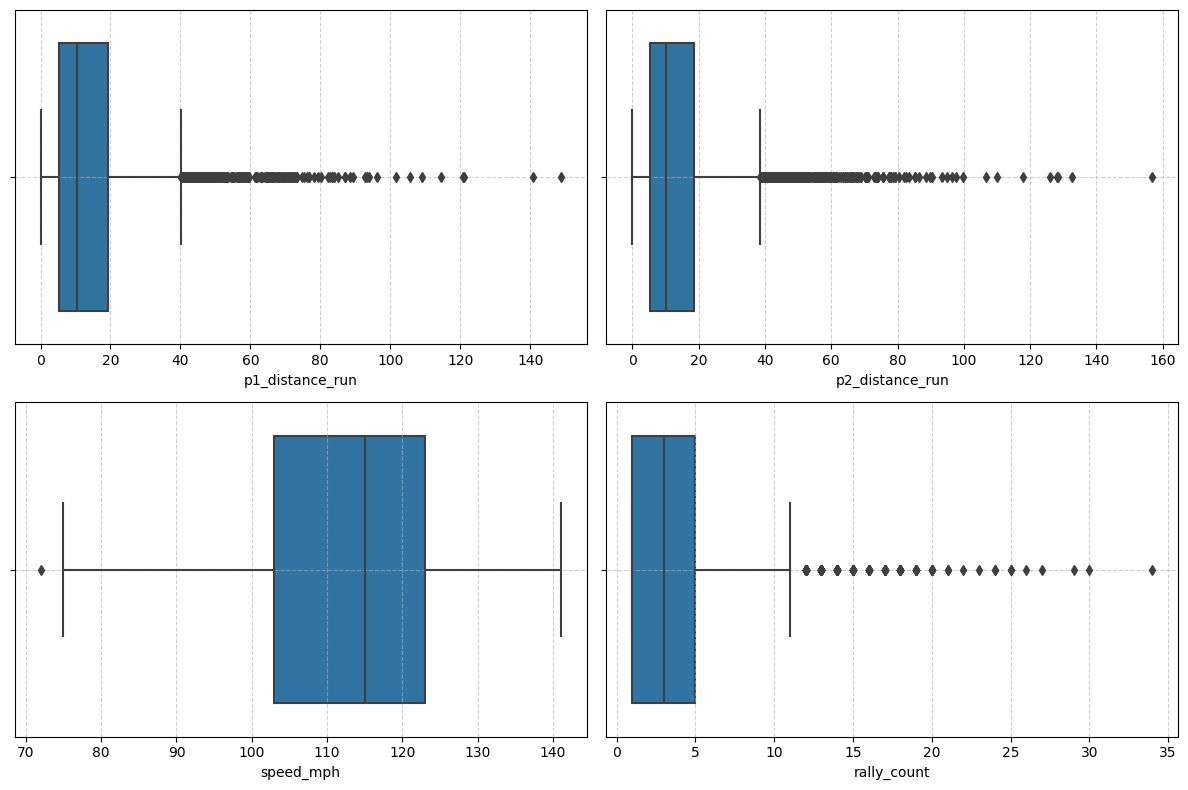
\includegraphics[width=0.75\textwidth,height = 0.45\textwidth]{boxplot.png}
    \caption{Boxplot of Each Variable}
    \label{fig:1}
\end{figure}

\pagebreak
According to the boxplot and the basic knowledge of tennis, we consider it not reasonable to have a rally count over 20 in a point, and for a player to run more than 100 meters in a point. 
Thus, we delete the rows in the dataset with a rally count over 20 and a distance run over 100. For the speed of the serve, all the values fall into a reasonable range, thus we didn't take any action on it.

Finally, we scale the dataset by the min-max normalization method. For min-max-normalize, we subtract the sample from the minimum of the data and then divide it by the difference between the maximum and minimum of the data, as the equation shows below.
\begin{equation}
    f(x) = \frac{x-min(x)}{max(x)-min(x)}
\end{equation}

\subsection{Method for Training Procedure}
%加一下哪里需要用training procedure
\quad For the training procedure in most of the training process, we applied the 5-fold cross-validation.
It's a statistical method used to evaluate the performance and stability of a predictive model or algorithm. 
It is particularly useful in scenarios where the available data is limited, and you want to estimate how well 
your model is likely to perform on unseen data. The process involves the following steps:
\begin{enumerate}
    \item Split the dataset into k subsets. Each subset is called a fold.
    \item For each unique group:
    \begin{enumerate}
        \item Take the group as a holdout or test data set
        \item Take the remaining groups as a training data set
        \item Fit a model on the training set and evaluate it on the test set
        \item Retain the evaluation score and discard the model
    \end{enumerate}
    \item Summarize the skill of the model using the sample of model evaluation scores
    \item The process is repeated k times, and the average of the k model evaluation scores is used as the estimate of the model's performance. 
    This average provides a more robust estimate of how the model is expected to perform on unseen data, as it incorporates multiple train-test splits.
\end{enumerate}

The advantage of using cross-validation is reducing the bias associated with a single random train-test split, providing a more accurate estimate of model performance.
It allows for the efficient use of available data, which is particularly beneficial when the dataset is limited in size. Every data point gets used for both training and validation across the folds.
Validating the model on different subsets of the data helps in identifying if the model is overfitting to a particular set of data and performs generality on the unseen data. Also, cross-validation helps in 
sensitivity analysis, which is the study of how the variation in the output of a model can be apportioned to different sources of variation in the input.

For the cross-validation specifically in our experiment, we sample the dataset into 5 folds based on the match ID to avoid a point played in the same match in both the training and validation set. 

\subsection{Model Assumption}
\quad To simplify the problem and feasibility of the model, we made the following assumptions:
\begin{enumerate}
    \item \textit{The statistics of the match are true and reliable.}
    \item \textit{The momentum of the player is more about the psychological state of the player, and the statistics of the match will reflect it.}
    \item \textit{All the players in the tournament tried their best to win the game and there is no match-fixing.}
    \item \textit{The existence of some extreme values in the dataset is reasonable.}
    \item \textit{The way we deal with the missing values and outliers is reasonable and will not affect the result of the model.}
\end{enumerate}

\subsection{Model Description}
\quad In this experiment, we used several machine learning models to predict the outcome of each point and capture the flow of play as points occur. The models we used are Light Gradient Boosting Machine (LGBM)\cite{GBM-model}, XGBoost\cite{XGB-model}, Support Vector Machine\cite{svm-model}, Multi-layer Perceptron\cite{multilayer-model} and Random Forest\cite{forest-model}.

Both LGBM and XGBoost are gradient-boosting decision tree models. The main advantage of these two models is their strong interpretability, as they can provide feature importance scores and decision nodes.
Thus, it's easy for us to understand and interpret how the match statistics reflect the performance of the player and use them to capture the momentum of the player. Also, they are in favor of handling small
datasets and have a fast training speed. Based on the size of the dataset and time constraints, we chose these two models as the main model for the experiment. Support Vector Machine is a powerful supervised 
learning model, especially in handling high dimensional data. Multi-layer Perceptron is a neural network model that can capture the non-linear relationship between the input and output. However, it may exist multiple
local minimums which highly depend on the weight initialization and it's hard to interpret the model. Random Forest has the basic advantages of tree models but it's likely to overfit the training data and also
time-consuming. 

Secondly, except for Multi-layer Perceptron, they are all able to be interpreted as we need to give some advice 
to the coach. In this sense, the Multi-layer Perceptron serves as a contrast sample to show if the interpretability of the model is deterministic in this task to some extent.


\section{Capture the Flow of Play}
\subsection{Prediction of the Outcome of Each Point}
\quad For the first question, we need to build a model that captures the flow of play as points occur and identify which player is performing better at a given time in the match. It should also quantify how much better they are performing\cite{pdf-tennis}.
Based on the dataset provided, we have mostly all the point-by-point data for the matches. To catch the flow of the play or in other words, the momentums of two players, we need to understand which variables significantly influence the outcome of each point. As there are more than 40 variables in the dataset, we need to perform a feature engineering on the current variables and select the variables that with a relatively high correlation with the outcome of the point. Based on this idea, we first come up with the following variables list in table \ref{table:2} as the indicator to predict the winner of that point, and all the variables concerning player 1. 
After standardizing these variables, as we described above, we use 5-fold cross-validation to train and validate each model. Figure \ref{fig:2} and Table \ref{table:3} demonstrate the result of the model performance.

\begin{table}[h!]
\centering
\begin{tabular}{||c c||} 
 \hline
 \textbf{Variable Name} & \textbf{Description} \\ [0.5ex] 
    \hline\hline
    $X_{1}$: gameWon & the number of games won in the current set \\ 
    \hline
    $X_{2}$: pointLeadG & the number of point leading in the current game \\
    \hline
    $X_{3}$: gameLeadS & the number of games leading in the current set \\
    \hline
    $X_{4}$: setLeadM & the number of sets leading in the current match  \\
    \hline
    $X_{5}$: ifServing & if the player is serving \\ 
    \hline
    $X_{6}$: ace & indicator of untouchable winning serve \\
    \hline
    $X_{7}$: winner & indicator of untouchable winning shot \\
    \hline
    $X_{8}$: dFault & indicator of double fault \\
    \hline
    $X_{9}$: unforcedE & indicator of unforced error \\
    \hline
    $X_{10}$: netPoints & the ratio of net points won in the current game \\
    \hline
    $X_{11}$: breakPoints & the ratio of break points won in the current set \\
    \hline
    $X_{12}$: distanceM & the total distance run in the current match \\
    \hline
    $X_{13}$: distanceLast3 & the total distance run in last 3 points \\
    \hline
    $X_{14}$: distanceCur & the distance run in the current point \\ 
    \hline
    $X_{15}$: speed & the speed of the last serve \\
    \hline
    $X_{16}$: trueSpeed & the product of $X_3$ and $X_{15}$ \\
    \hline
    $X_{17}$: rallyCur & the rally count of the current point \\
    \hline
    $X_{18}$: rallyLast3 & the average of rally count in the last 3 points \\
    \hline
    $X_{19}$: pointsLast3 & the point won by player 1 in last 3 points \\
    [1ex] 
    \hline
\end{tabular}
\caption{Variables' Name and Description}
\label{table:2}
\end{table}

\begin{table}[h!]
\centering
\begin{tabular}{||c c c c c c||} 
 \hline
 \textbf{Model} & \textbf{Accuracy} & \textbf{Recall} & \textbf{Precision} & \textbf{F1} & \textbf{AUC} \\ [0.5ex] 
 \hline\hline
 LGBM & 0.91 & 0.92 & 0.91 & 0.92 & 0.97 \\ 
 \hline
 XGBoost & 0.91 & 0.92 & 0.90 & 0.91 & 0.97 \\
 \hline
 SVM & 0.89 & 0.89 & 0.89 & 0.89 & 0.96 \\
 \hline
 MLP & 0.91 & 0.91 & 0.91 & 0.91 & 0.97 \\
 \hline
 Random Forest & 0.91 & 0.91 & 0.91 & 0.91 & 0.97 \\
 [1ex] 
 \hline
\end{tabular}
\caption{Model Performance}
\label{table:3}
\end{table}

\begin{figure}[!h]
    \centering
    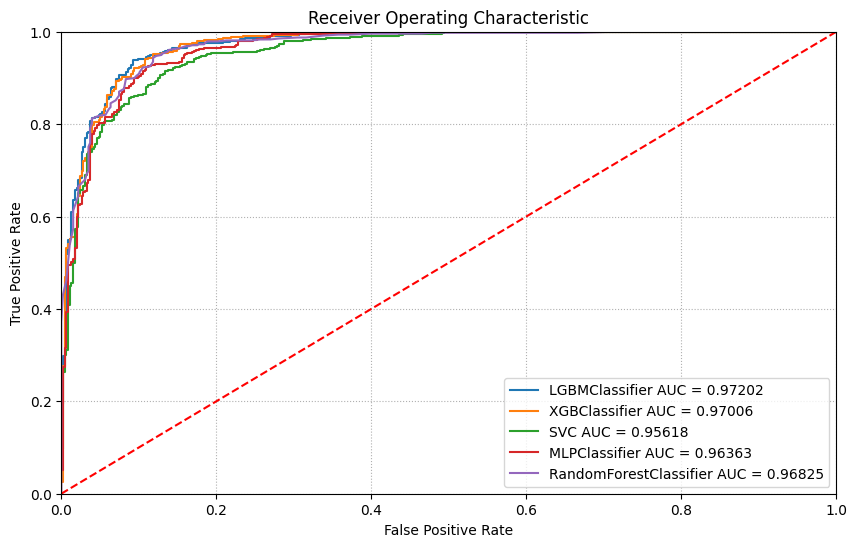
\includegraphics[width=0.6\textwidth, height=0.4\textwidth]{auc.png}
    \caption{AUC of Different Models}
    \label{fig:2}
\end{figure}

Based on the result, we can see both LGBM and XGBoost have the best performance in predicting the outcome of each point. As we used 5-fold cross-validation in the training process, the high F1 score also indicates the robustness of LGBM and XGBoost under different training data. In the next step, we extract
the feature importance of these two models as figure  \ref{fig:3} and \ref{fig:4} show and further select the variable to quantify the momentum of the player.

\begin{figure}[h!]
    \centering
    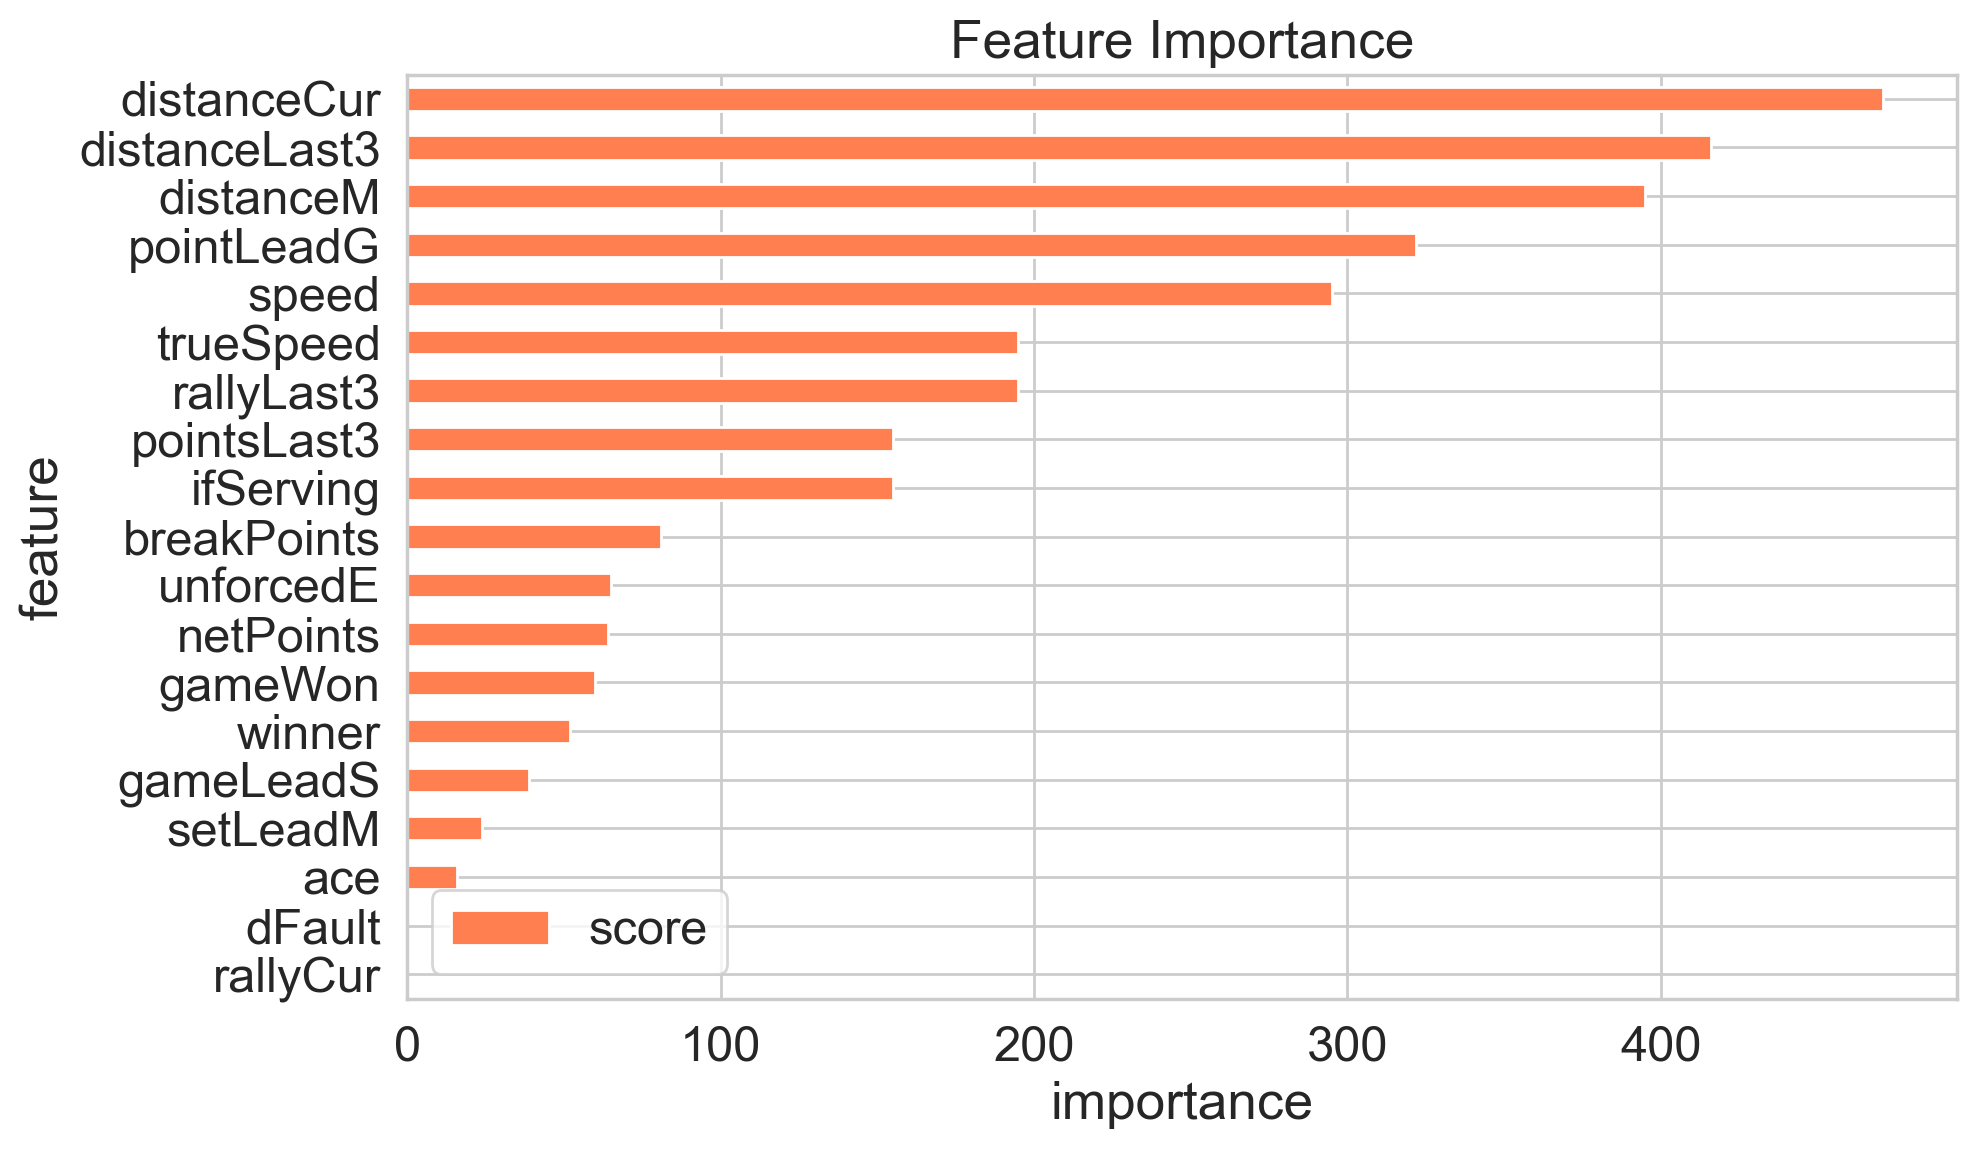
\includegraphics[width=0.8\textwidth]{feature_LGBM.png}
    \caption{Feature Importance of LGBM}
    \label{fig:3}
\end{figure}

\begin{figure}[h!]
    \centering
    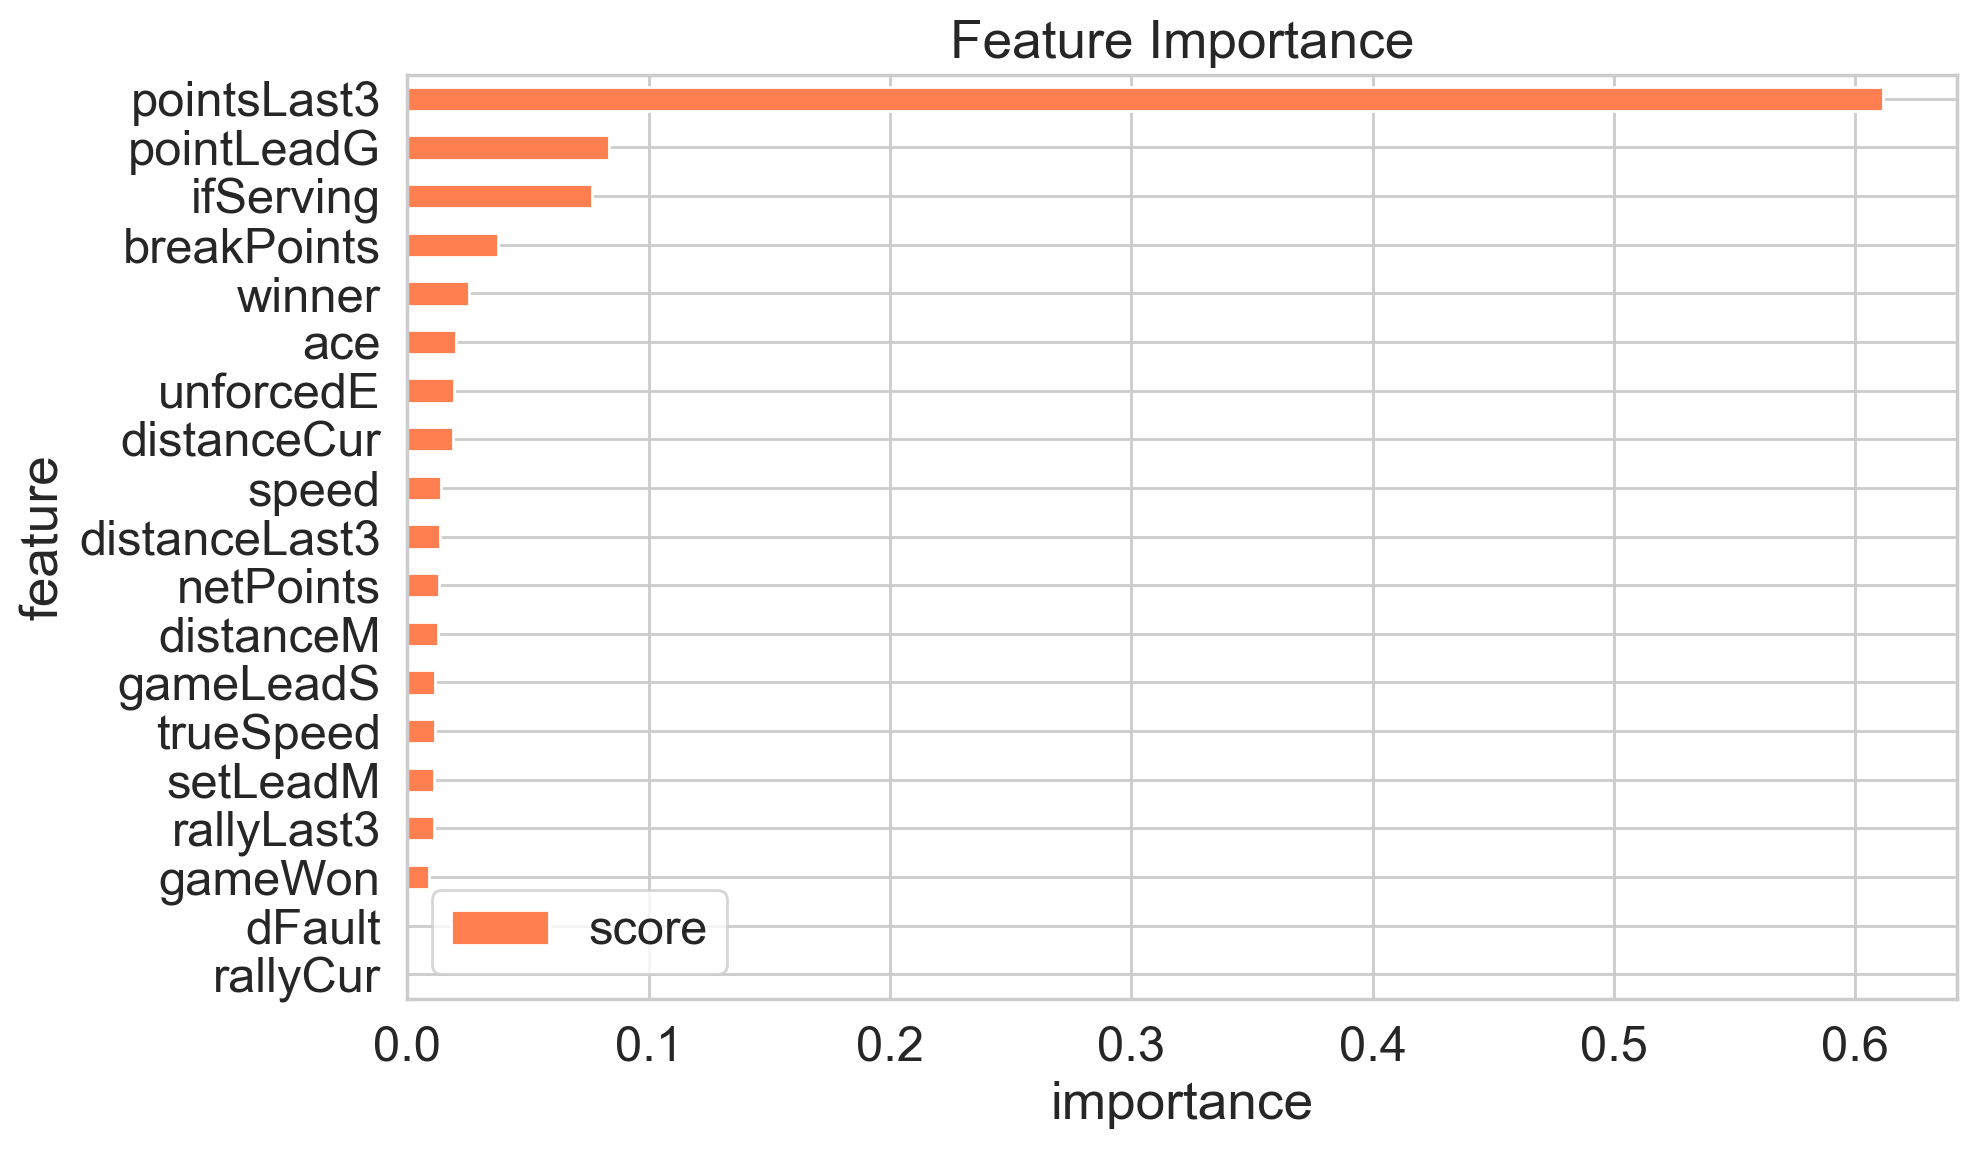
\includegraphics[width=0.8\textwidth]{feature_XGB.png}
    \caption{Feature Importance of XGBoost}
    \label{fig:4}
\end{figure}

\pagebreak
\subsection{Quantify the Momentum of the Player}
\quad Based on the feature importance, we can see the performance on the last 3 points of the game has a crucial importance in predicting the current play. Therefore, we decide to use the rolling average of variables in the last 3 games to capture the momentum of a player.
According to the feature importance we extract from the LGBM and XGBoost model, we select the variables (refer to the appendix) that have the most influential statistics on a player's momentum, and develop our algorithm
to quantify the momentum of the player. 

The algorithm first sums up each of the selected variables in the last 3 points of both players. We call each of the
the sum of variables as the criteria.

\begin{figure}[h!]
    \centering
    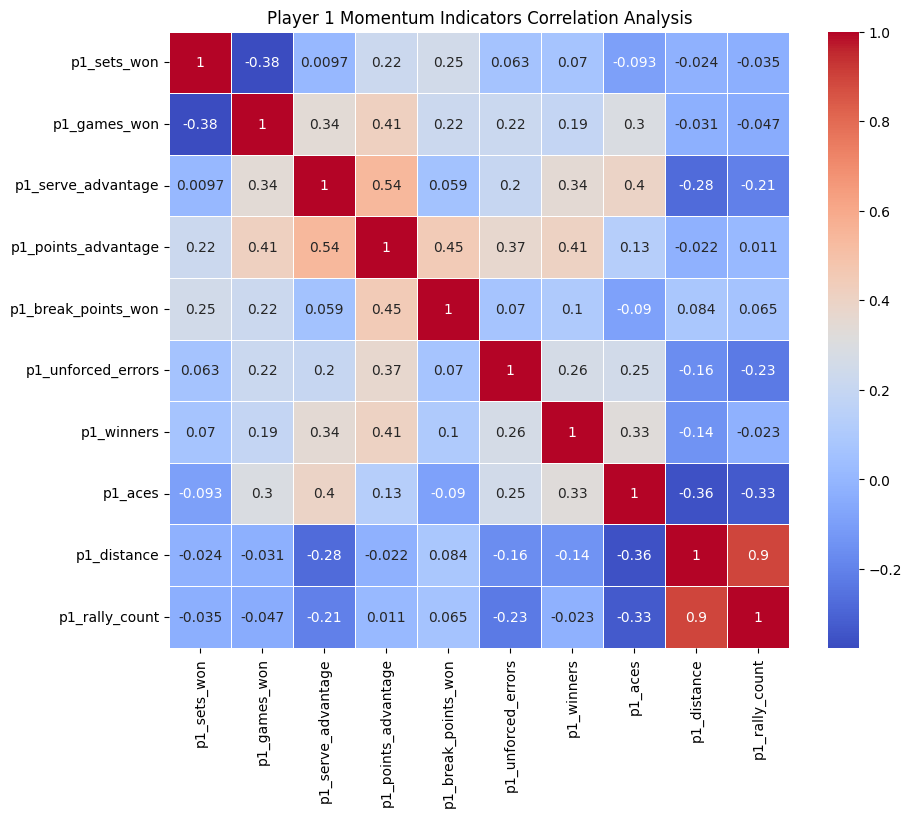
\includegraphics[width=0.7\textwidth]{correlation.png}
    \caption{Correlation Matrix of Each Criterion of Player 1 in the Final of Wimbledon 2023} 
    \label{fig:5}
\end{figure}

\begin{figure}[h!]
    \centering
    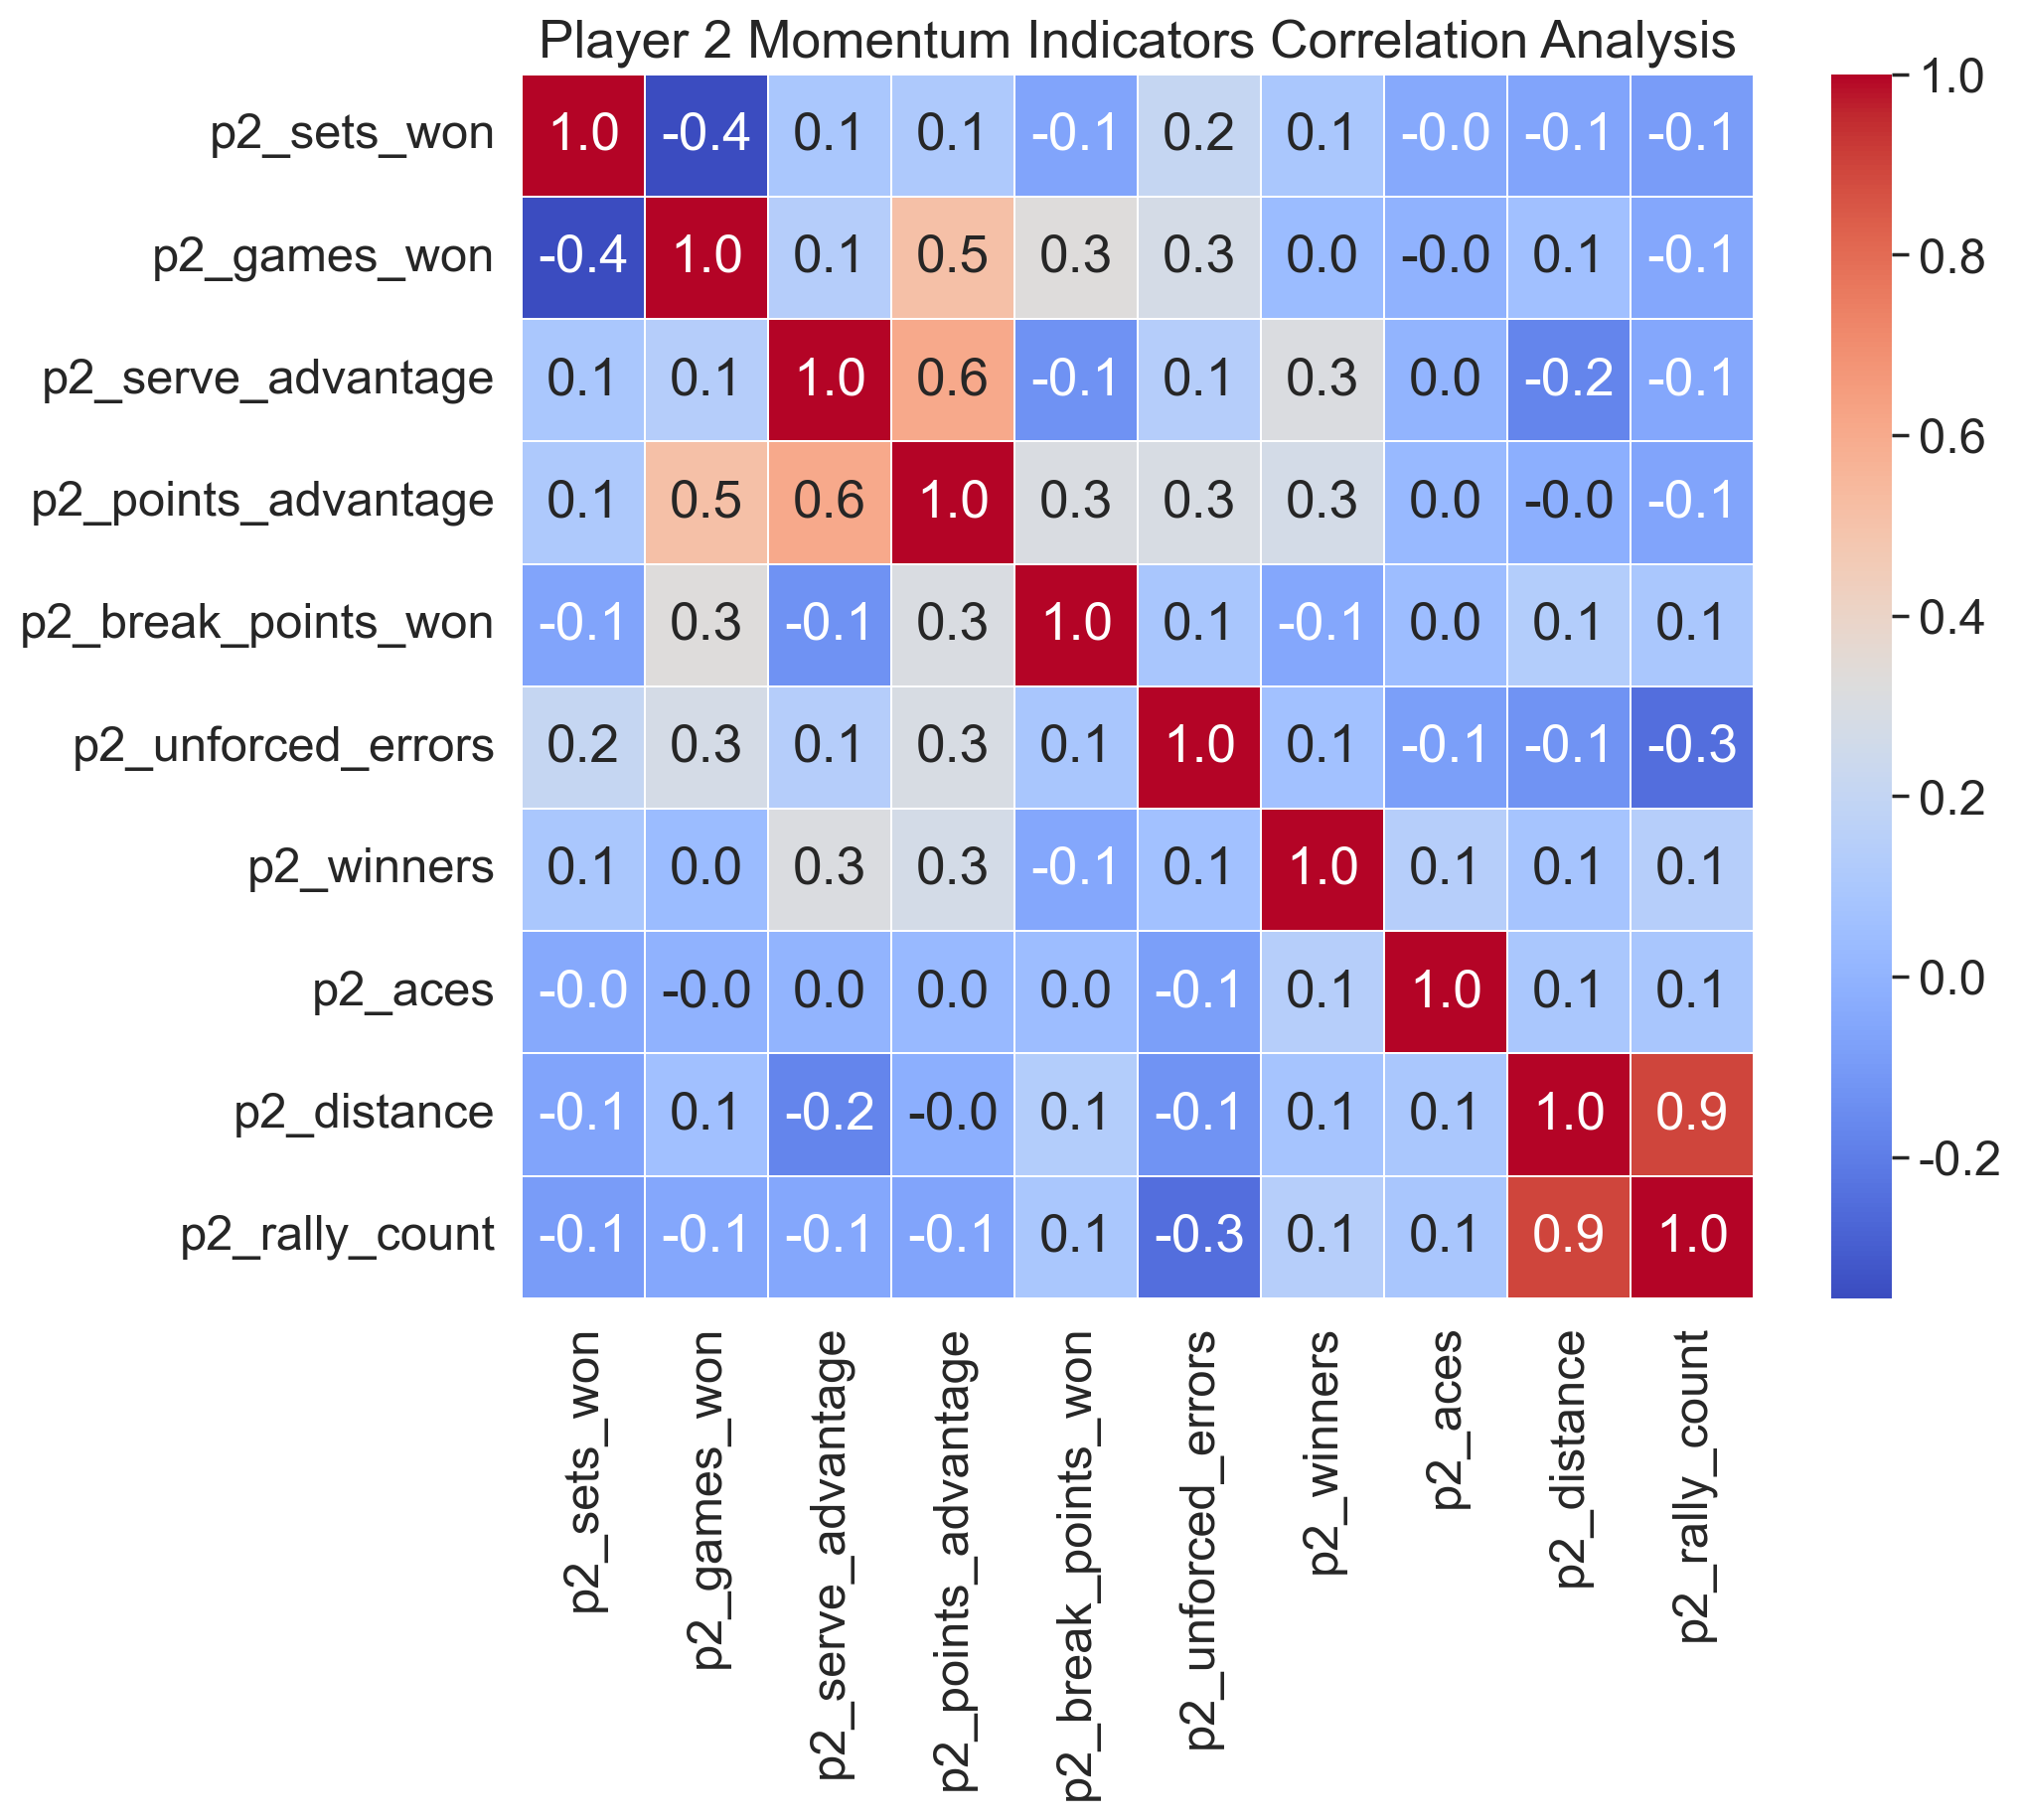
\includegraphics[width=0.7\textwidth]{correlation_2.png}
    \caption{Correlation Matrix of Each Criterion of Player 2 in the Final of Wimbledon 2023} 
    \label{fig:6}
\end{figure}

Figure \ref{fig:5} is the heatmap of the correlation matrix of each criterion of both players in the final of Wimbledon 2023. After we get the criteria, we apply the entropy weight method to assign weight to each variable and then sum them up to get the momentum of the player. 
The entropy weight method is a multi-criteria decision-making method. In the specific use of the process, the entropy weighting method according to the degree of 
variability of the indicators, the use of information entropy to calculate the entropy of the indicators, and then through the entropy of the weight of the 
indicators to correct, to get a more objective weight of the indicators. The entropy weight method works as follows:

\begin{enumerate}
    \item Normalize the data under each criterion (indicator) by min-max normalization.
    \begin{equation}
        Y_{ij} = \frac{X_{ij}-min(X_i)}{max(X_i)-min(X_i)}
    \end{equation} where $Y_{ij}$ is the normalized value of the $j$th criteria of 
    the $i$th sample, $X_{ij}$ is the original value of the $j$th criteria of the $i$th data sample, $min(X_i)$ and $max(X_i)$ are the minimum and maximum value of the $i$th indicator.
    \item 
    \begin{equation}
        P_{ij} = \frac{Y_{ij}}{\sum_{i=1}^{n}Y_{ij}}
    \end{equation} where $P_{ij}$ is the proportion of the $i$th data sample in the $j$th criteria, $Y_{ij}$ is the normalized value of the $j$th criteria of the $i$th sample, $n$ is the number of data samples.
    \item Calculate the entropy of the $j$th criteria.
    \begin{equation}
        E_j = -\frac{1}{\ln(n)}\sum_{i=1}^{n}P_{ij}\ln(P_{ij})
    \end{equation} where $E_j$ is the entropy of the $j$th criteria, $P_{ij}$ is the proportion of the $i$th data sample in the $j$th criteria, $n$ is the number of data samples.
    \item Calculate the weight of the $j$th criteria.
    \begin{equation}
        W_j = \frac{1-E_j}{\sum_{j=1}^{m}(1-E_j)}
    \end{equation} where $W_j$ is the weight of the $j$th criteria, $E_j$ is the entropy of the $j$th criteria, $m$ is the number of criteria.
\end{enumerate}

The weighted sum of the criteria is the momentum of the player. Again, we select the final of Wimbledon 2023 as an example to show the momentum of each player.
\begin{figure}[h!]
    \centering
    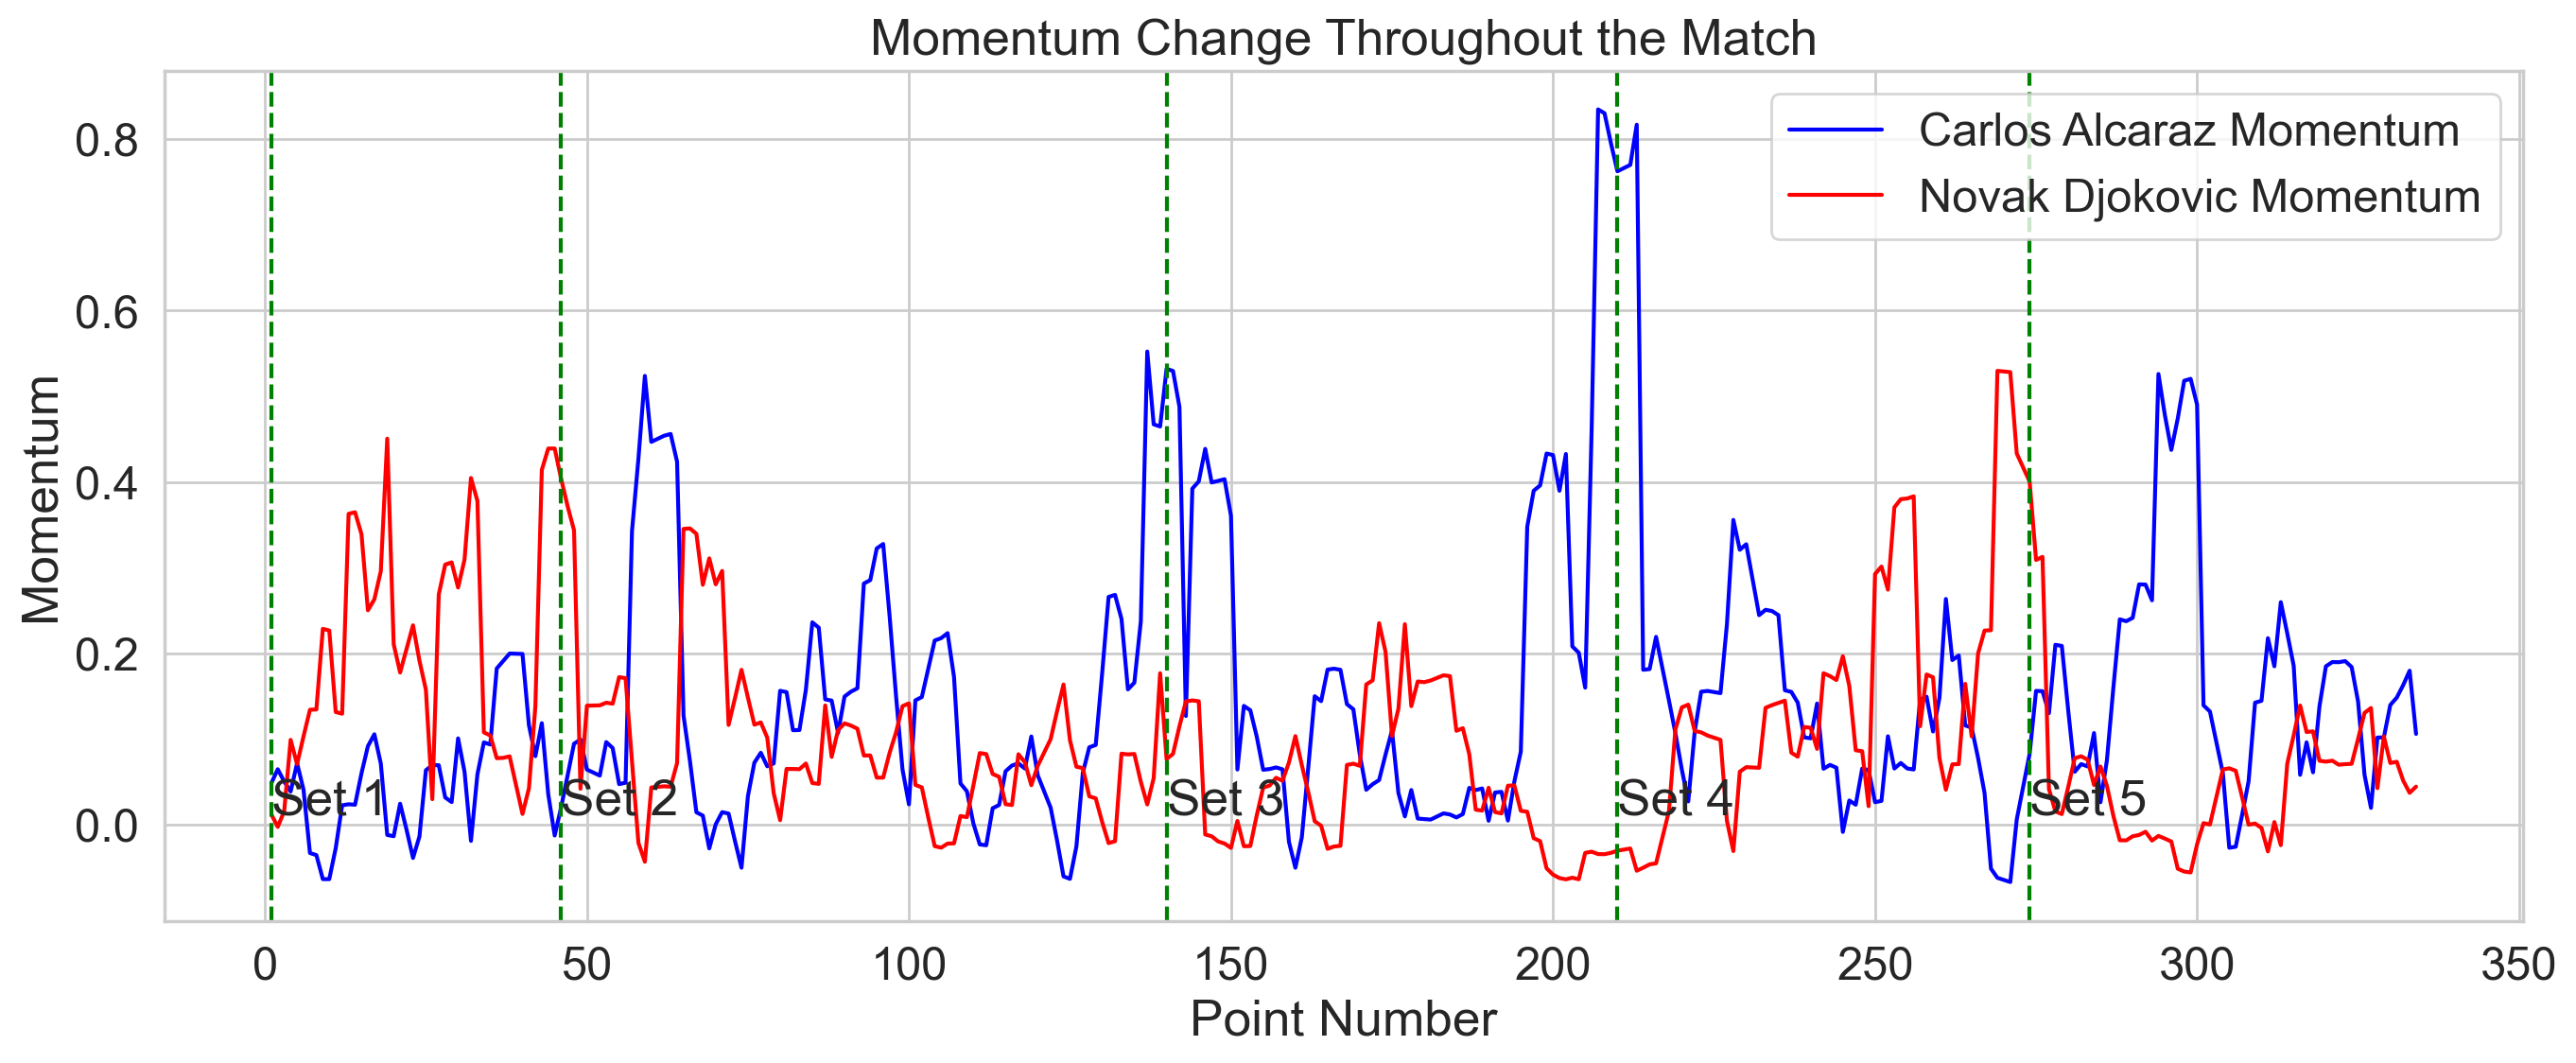
\includegraphics[width=0.9\textwidth]{flow.png}
    \caption{Momentum of Each Player in the Final of Wimbledon 2023} 
    \label{fig:7}
\end{figure}

According to figure\ref{fig:7}, the flow of the match is captured by the momentum of each player. As Djokovic 
dominated the first set 6 to 1, we can see his momentum was much higher than Alcaraz's almost all the time in the first set.
The second set was much more competitive, the momentums of both players fluctuated alternately. Also, as Alcaraz got the 
tiebreak, we can observe his momentum at the end of the second set had a significant increase and he brought it into the 
third set and won with 6 to 1. The momentum during the fourth set also captured what exactly happened in the match, Alcaraz
controlled the first part and Djokovic reversed the game. The situation in the final set was also described by the momentum.
Based on the result, we can see after selecting the important feature by applying the entropy weight method, we can use the momentum
to capture the flow of play as points occur and identify which player is performing better at a given time in the match, as well as 
the numerical value of momentum can quantify how much better they are performing.

\section{Verify the Statistical Significance of Momentum}
\quad To prove the swing of the play and the momentum are not just random, we performed an ordinary least square regression on the 19 variables
we selected in the previous part and the outcome of the point. As the R square of the regression is 0.9, we can see the 19 variables are
highly correlated with the outcome of the point.

We then performed Z-Score normalization and calculated the 
p-value of the momentum of each player in each round of the Wimbledon 2023 tournament. Beyond that, we also write an algorithm to
detect the swing of the play by calculating the turning point of the momentum as figure \ref{fig:14}. 

\begin{figure}[h!]
    \centering
    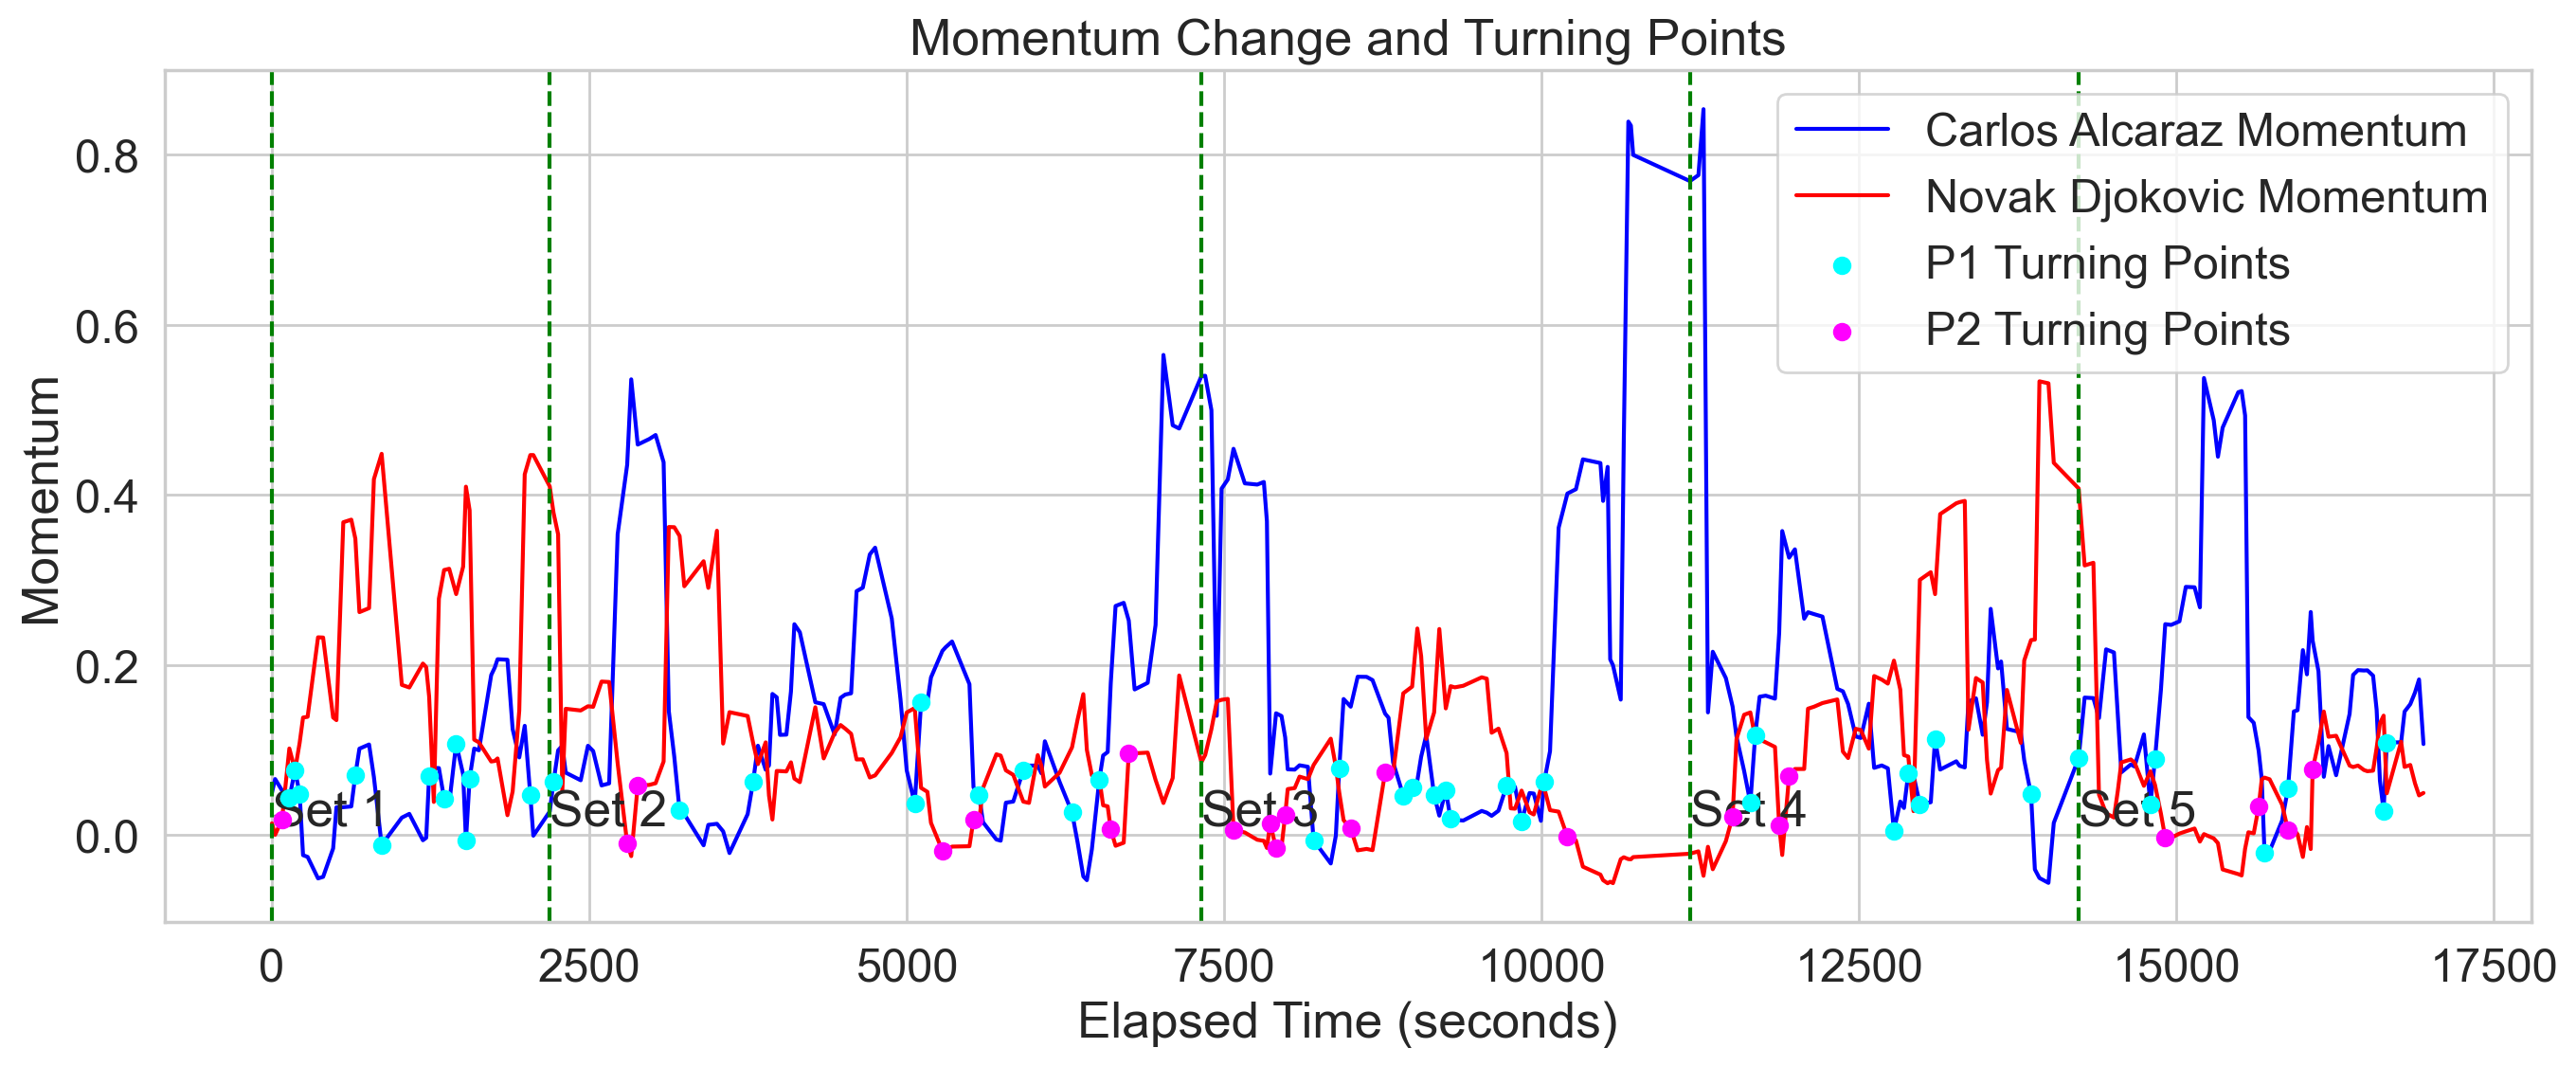
\includegraphics[width=0.9\textwidth]{turning_point.png}
    \caption{Turing Points in the Final of Wimbledon 2023} 
    \label{fig:14}
\end{figure}

We also perform a t-test to verify the statistical
significance of the turning point. For each match, if the p-value of the momentum is less than 0.05, we indicate it as 1 meaning the
momentum is significant, otherwise, we indicate it as 0. And the same for the turning point. The result is shown in the table \ref{table:3}.
\begin{table}[h!]
\centering
\begin{tabular}{|| c c c c c ||}
    \hline 
    \textbf{Stats} & \textbf{P1 momen} & \textbf{P2 momen} & \textbf{P1 turning} & \textbf{P2 turning} \\ [0.5ex] 
    \hline\hline
    mean & 1.000 & 1.000 & 0.379 & 0.448 \\
    \hline
    std & 0.000 & 0.000 & 0.494 & 0.506 \\
    [1ex]
    \hline
\end{tabular}
\caption{Summary of T Test Result}
\label{table:4}
\end{table}

Based on the result, we can see for each match, the momentums of both players are statistically significant. However, for the turning point,
both of them have less than $50\%$ of the matches are statistically significant. The reason might arise from the fact that the swing of the play
may not directly occur right after the turning point of momentum. Although the turning point of the momentum is not statistically significant, we 
still confirm that the momentum of each player is statistically significant which means runs of success by one player are not random.

\section{Indicator of the Flow of Play}
\subsection{Model Selection}
\quad As we verified the momentum of each player is statistically significant, the prediction of momentum becomes a crucial part of the match analysis.
If the coach can capture the momentum of the player as the match proceeds, then he can give some insightful advice to the player to either keep the momentum or 
reverse the game. Hence in this part, we set the difference of the momentum of a player in the current point and the next point as the target variable to predict.
We use the same 19 variables as the input to predict the difference in the momentum. We sample one match from the dataset and use the XGBoost model and CNN-LSTM\cite{graph-tennis} model to predict
the difference in the momentum. The reason for choosing XGBoost is simple it's the performed model in the previous part. Additionally, we want to capture the time series
relationship between each point, and CNN-LSTM is good at capturing the temporal relationship of the input data. 

\begin{figure}[h!]
    \centering
    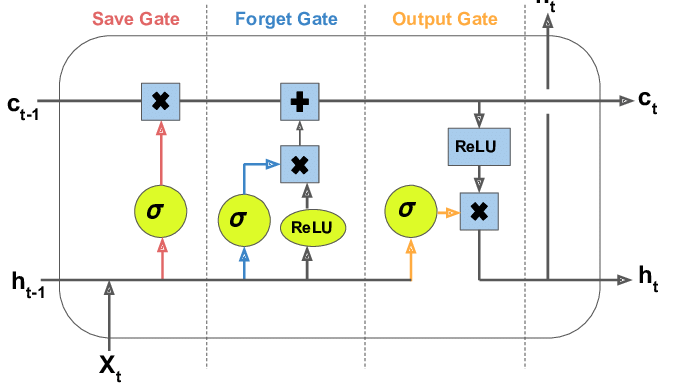
\includegraphics[width=0.6\textwidth, height=0.4\textwidth]{LSTM.png}
    \caption{Structure of LSTM\cite{graph-tennis}} 
    \label{fig:15}
\end{figure}

\subsection{Model Performance and Evaluation}
We selected 2023 Wimbledon-1701 as the sample match to predict the difference in the momentum. We use the first 80\% of the match as the training set and the rest as the validation set.
We use the mean absolute percentage error as the evaluation metric. The results for XGBoost and CNN-LSTM are $8.476\%$ and $4.389\%$ respectively. The results for both models are shown in the figure  \ref{fig:8} and \ref{fig:9}.
\begin{figure}[h!]
    \centering
    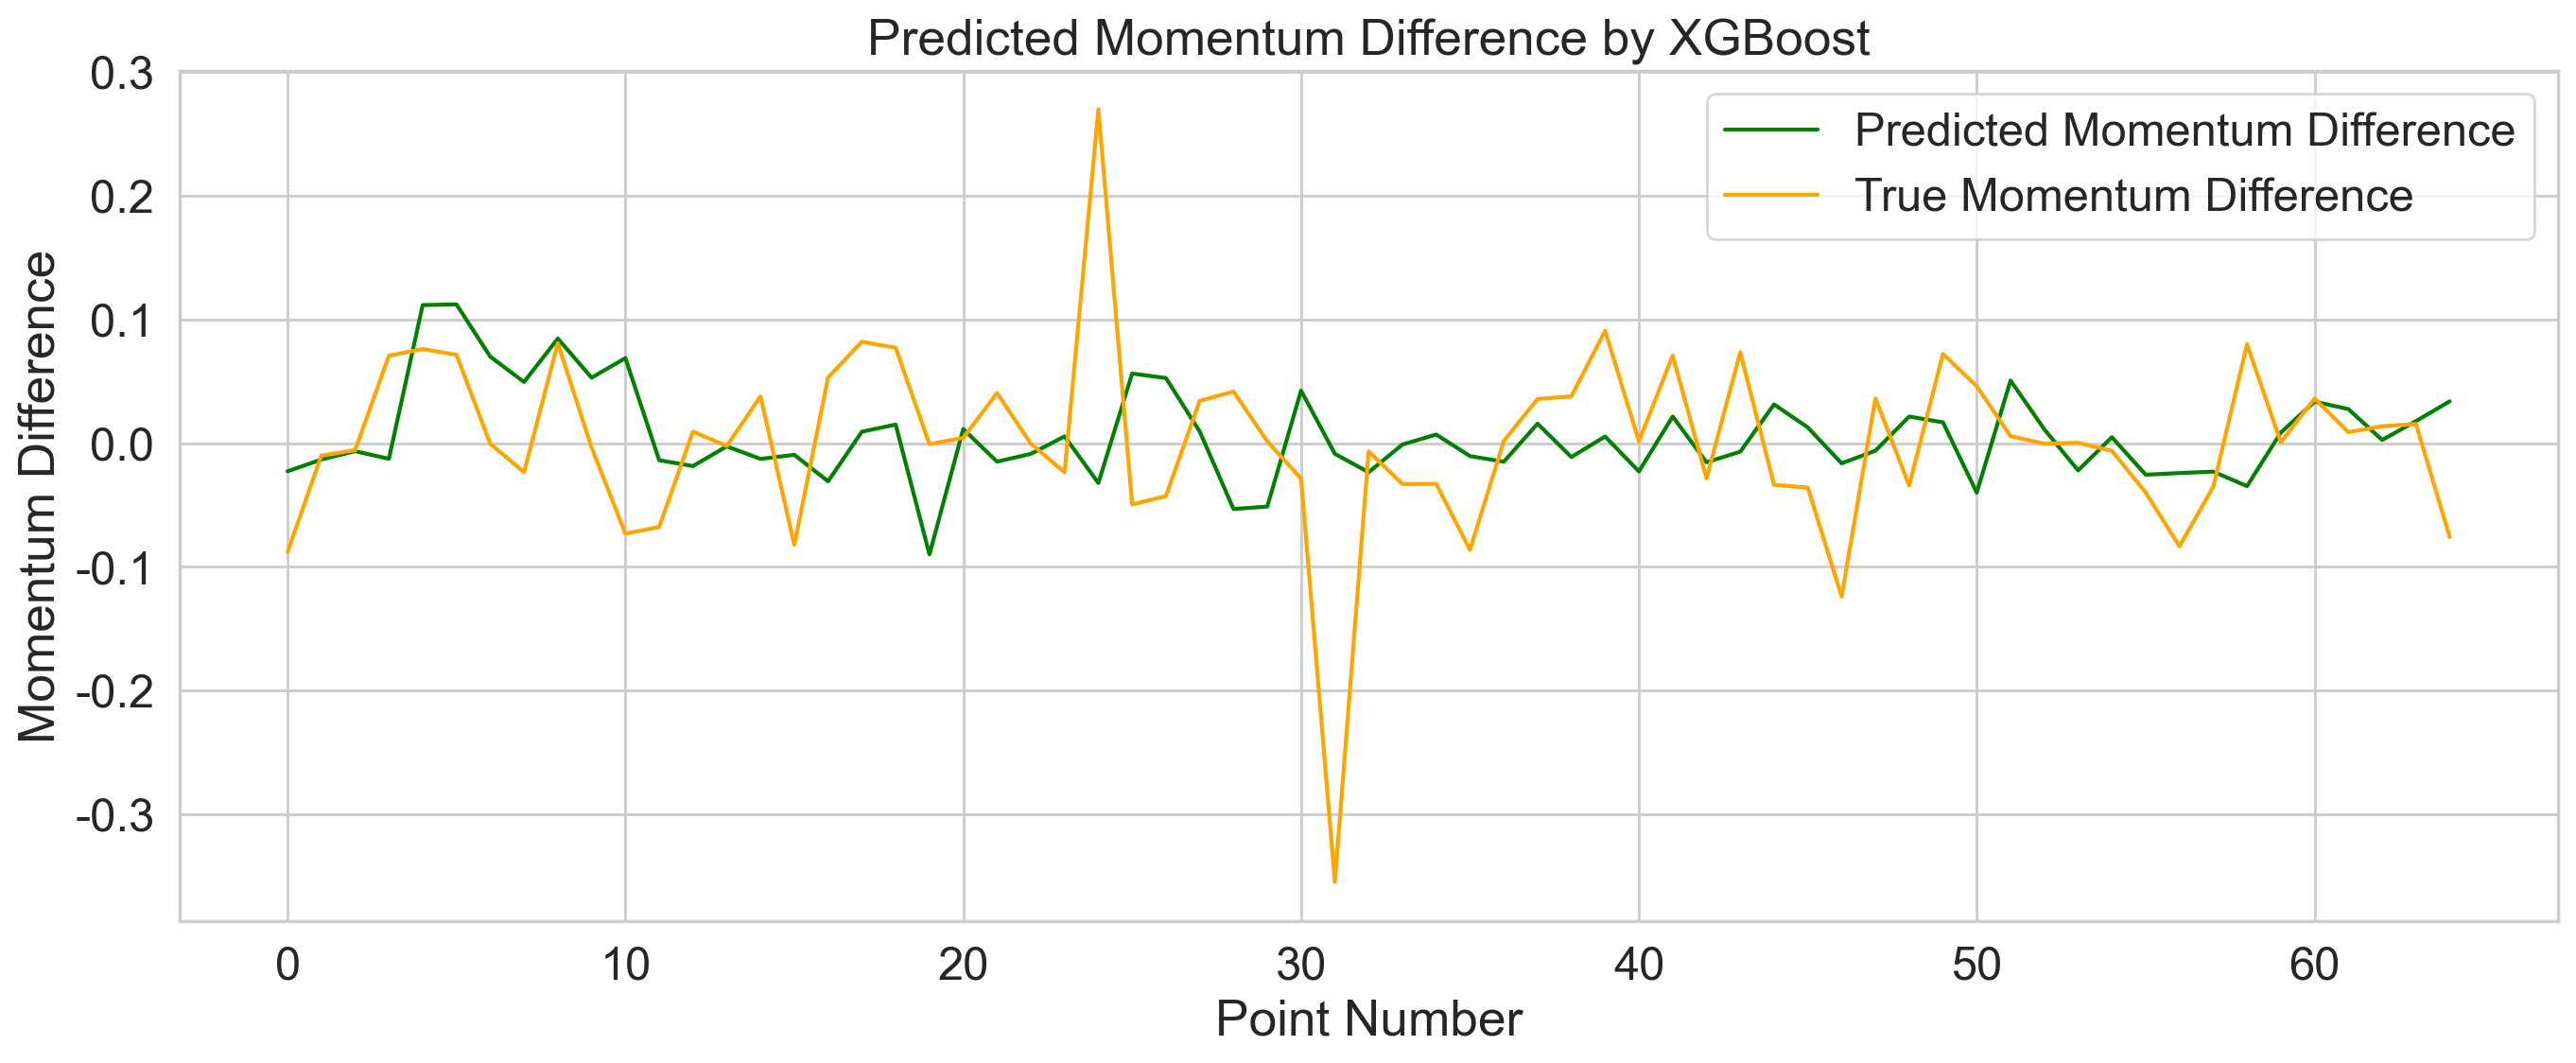
\includegraphics[width=0.7\textwidth, height=0.3\textwidth]{XGboost_part_3.png}
    \caption{Prediction of the Difference of the Momentum by XGBoost}
    \label{fig:8}
\end{figure}

\begin{figure}[h!]
    \centering
    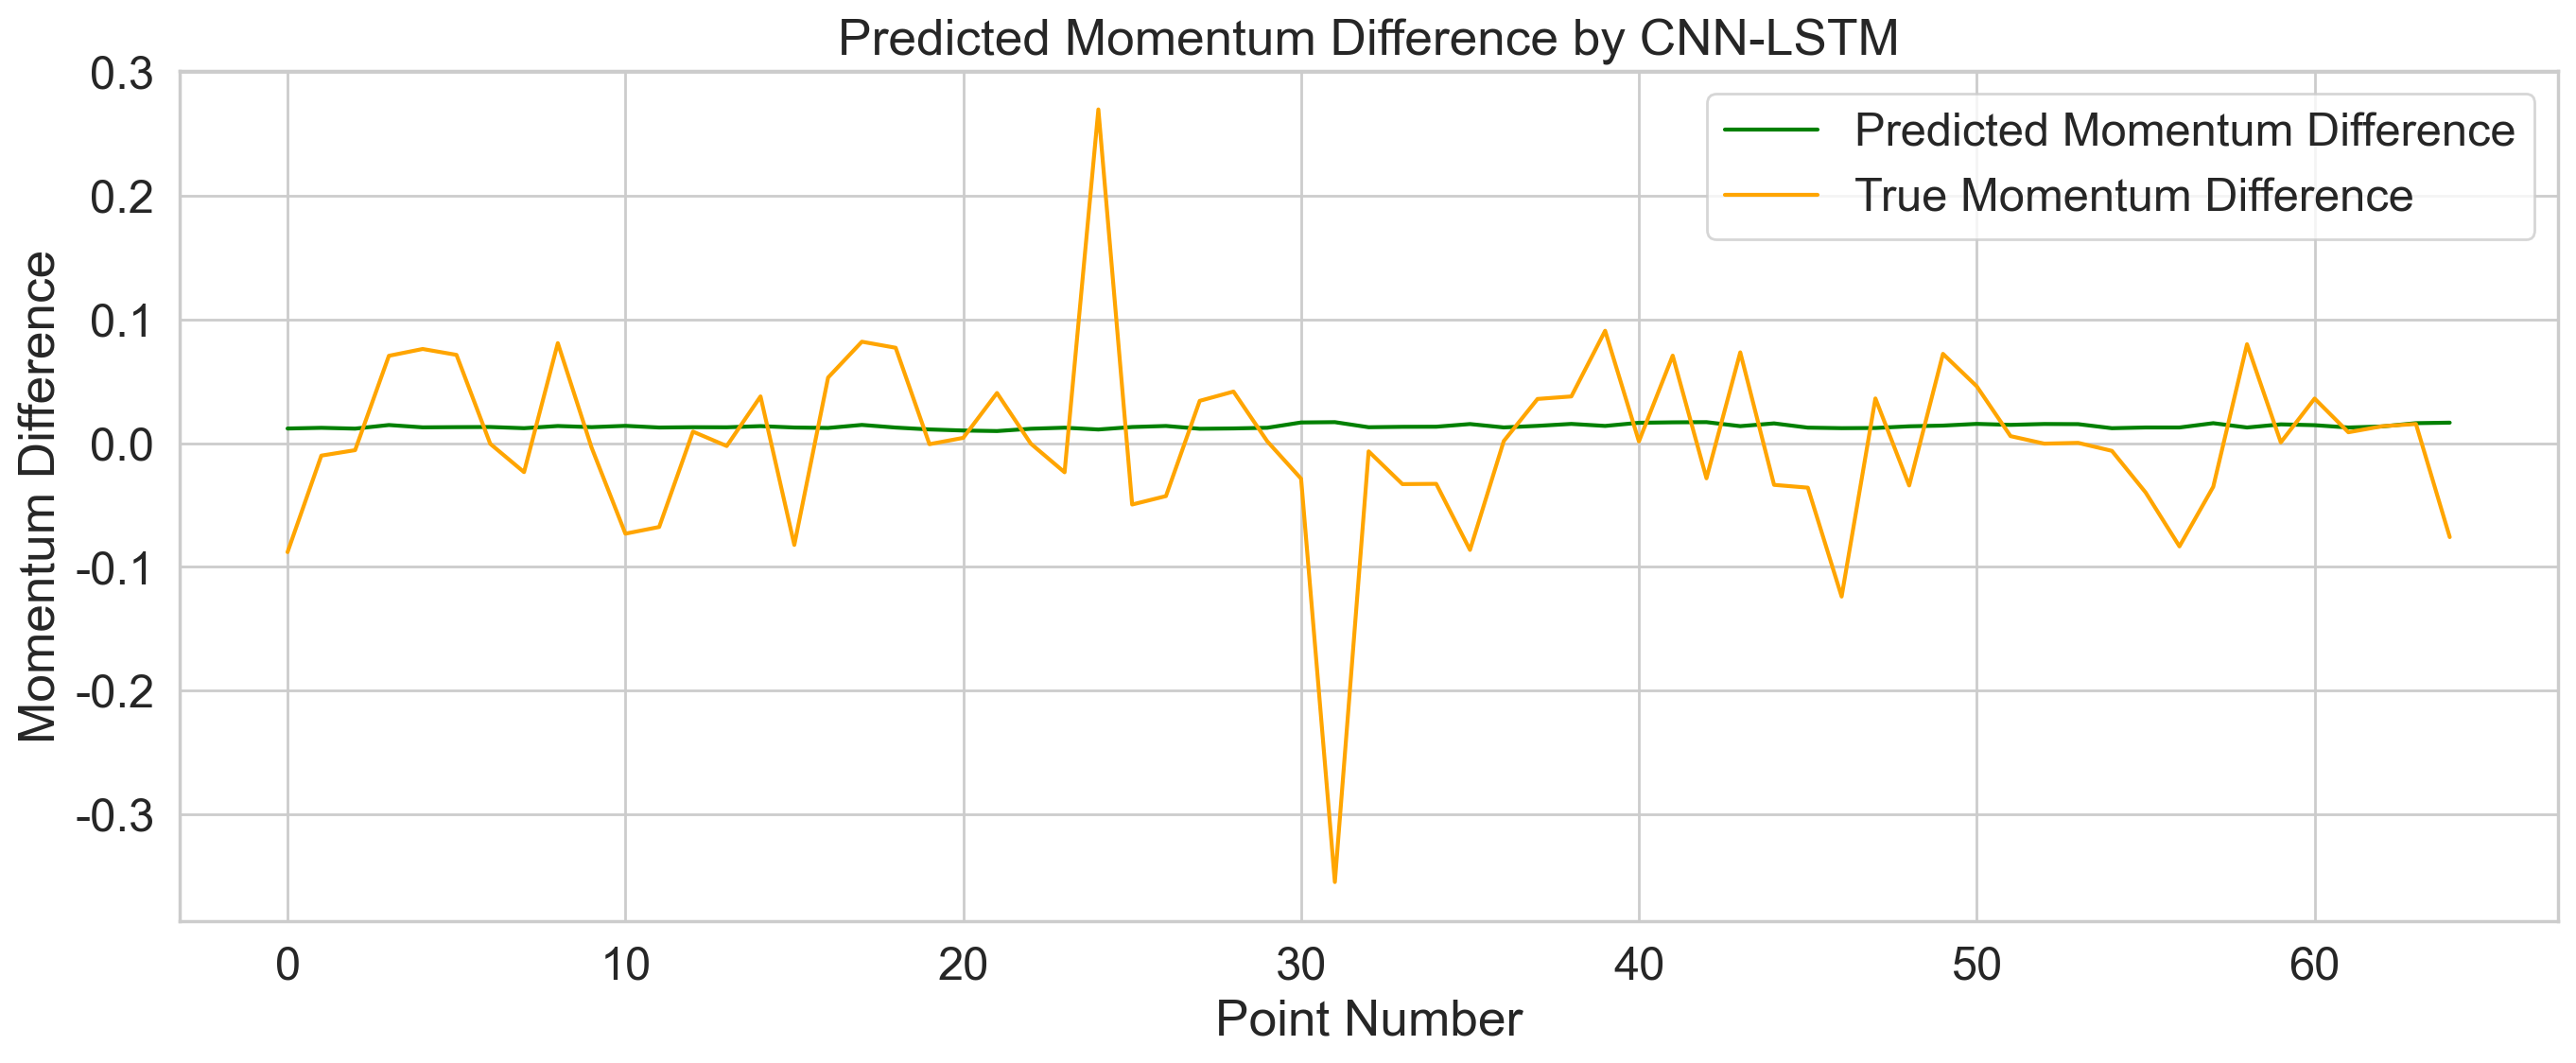
\includegraphics[width=0.7\textwidth, height=0.3\textwidth]{CNNLSTM_part_3.png}
    \caption{Prediction of the Difference of the Momentum by CNN-LSTM}
    \label{fig:9}
\end{figure}

Based on the result, we can see that XGBoost catches the trend of the difference of the momentum, although the mean absolute percentage error is a little bit higher. 
Therefore, we plot the features that have the highest importance in the XGBoost that determine the difference of the momentum in two consecutive points as figure  \ref{fig:10} shows.
\begin{figure}[h!]
    \centering
    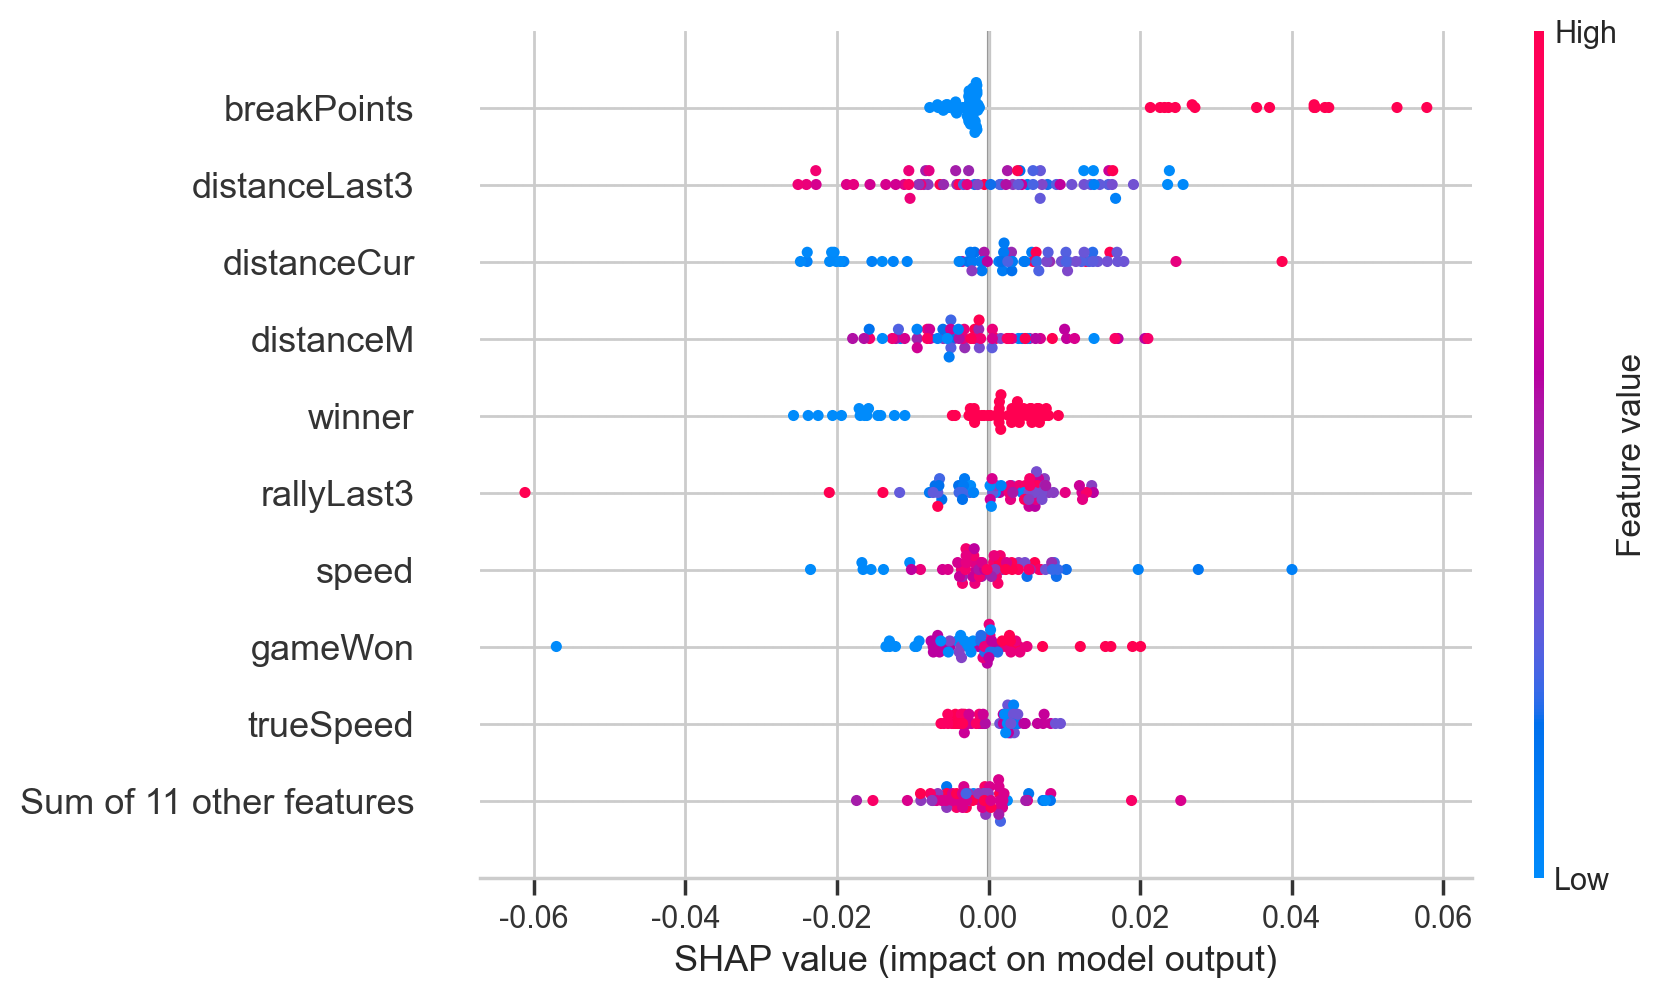
\includegraphics[width=0.9\textwidth, height=0.5\textwidth]{determinstic_value.png}
    \caption{Feature Importance of XGBoost for Selected Match}
    \label{fig:10}
\end{figure}

\begin{figure}[h!]
    \centering
    \includegraphics[width=0.9\textwidth, height=0.5\textwidth]{XGboost_match.png}
    \caption{Feature Importance of XGBoost in Tournament}
    \label{fig:11}
\end{figure}

Based on the mean absolute percentage error and the plot, we can see it hard to predict the increase or decrease of the momentum of the player exactly. However, through the
plot, we can see that the XGBoost model follows the trend of the change of momentum to some extent. Therefore, extracting the features that have the highest impact on predicting the 
difference in momentum can still provide some insightful advice to the coach. 

Through that plot we can see that to have a strong momentum during the game, it's important to catch the chance of the break points. As the statistics show, the breakpoints are the most 
influential feature to have a positive impact on the momentum. Therefore, the coach should pay attention to how to guide the player to win the breakpoints as it will not only help boost the 
momentum of the player but also build the player's morale and confidence. Moreover, the coach should also keep in mind the distance and rally count. They are the indicators of the
physical exertion of players. Too much distance run and rally count may lead to the fatigue of the player and thus decrease the momentum. Finally, an untouchable winning shot also contributes positively to the momentum, it is a good reflection of the player's ability to read the game and catch the weakness of the opponent.

To give the player some advice to prepare for the new game, we also trained the model with the $80\%$ of the matches during the Wimbledon 2023 tournament and used the rest $20\%$ as the validation set, and we 
ensured that all the matches in the training set are not in the validation set. The mean absolute percentage error is $6.191\%$ for the XGBoost model and $5.179\%$ for the CNN-LSTM model. Figure \ref{fig:11} 
shows how each feature contributes to predicting the difference in the momentum. Through the plot, we can see that in a more general case, the points lead plays a more important role besides break points. However, counter-intuitively, we can observe from the plot that samples both contribute positively and negatively to the momentum. We think it might depend on the psychological states of different players. Some of them might feel relaxed after getting the lead and make errors.
Therefore to prepare a new game,
the player needs to be cautious when he gets the lead of the game to hold a strong momentum. More than that, the serve advantage becomes more clear in the general case. Therefore, the coach should also notice the 
player to catch each change of serving advantage in order to have a better chance to win the game.

\section{The Generality of the Model}
\quad To test the generality and sensitivity of the model we used to predict the difference of the momentum, we randomly
sampled 6 matches from the dataset and used both XGBoost and CNN-LSTM to predict the difference of the momentum. Figure \ref{fig:12}
and \ref{fig:13} shows the result of the prediction of the difference of the momentum by XGBoost and CNN-LSTM.

\begin{figure}[h!]
    \centering
    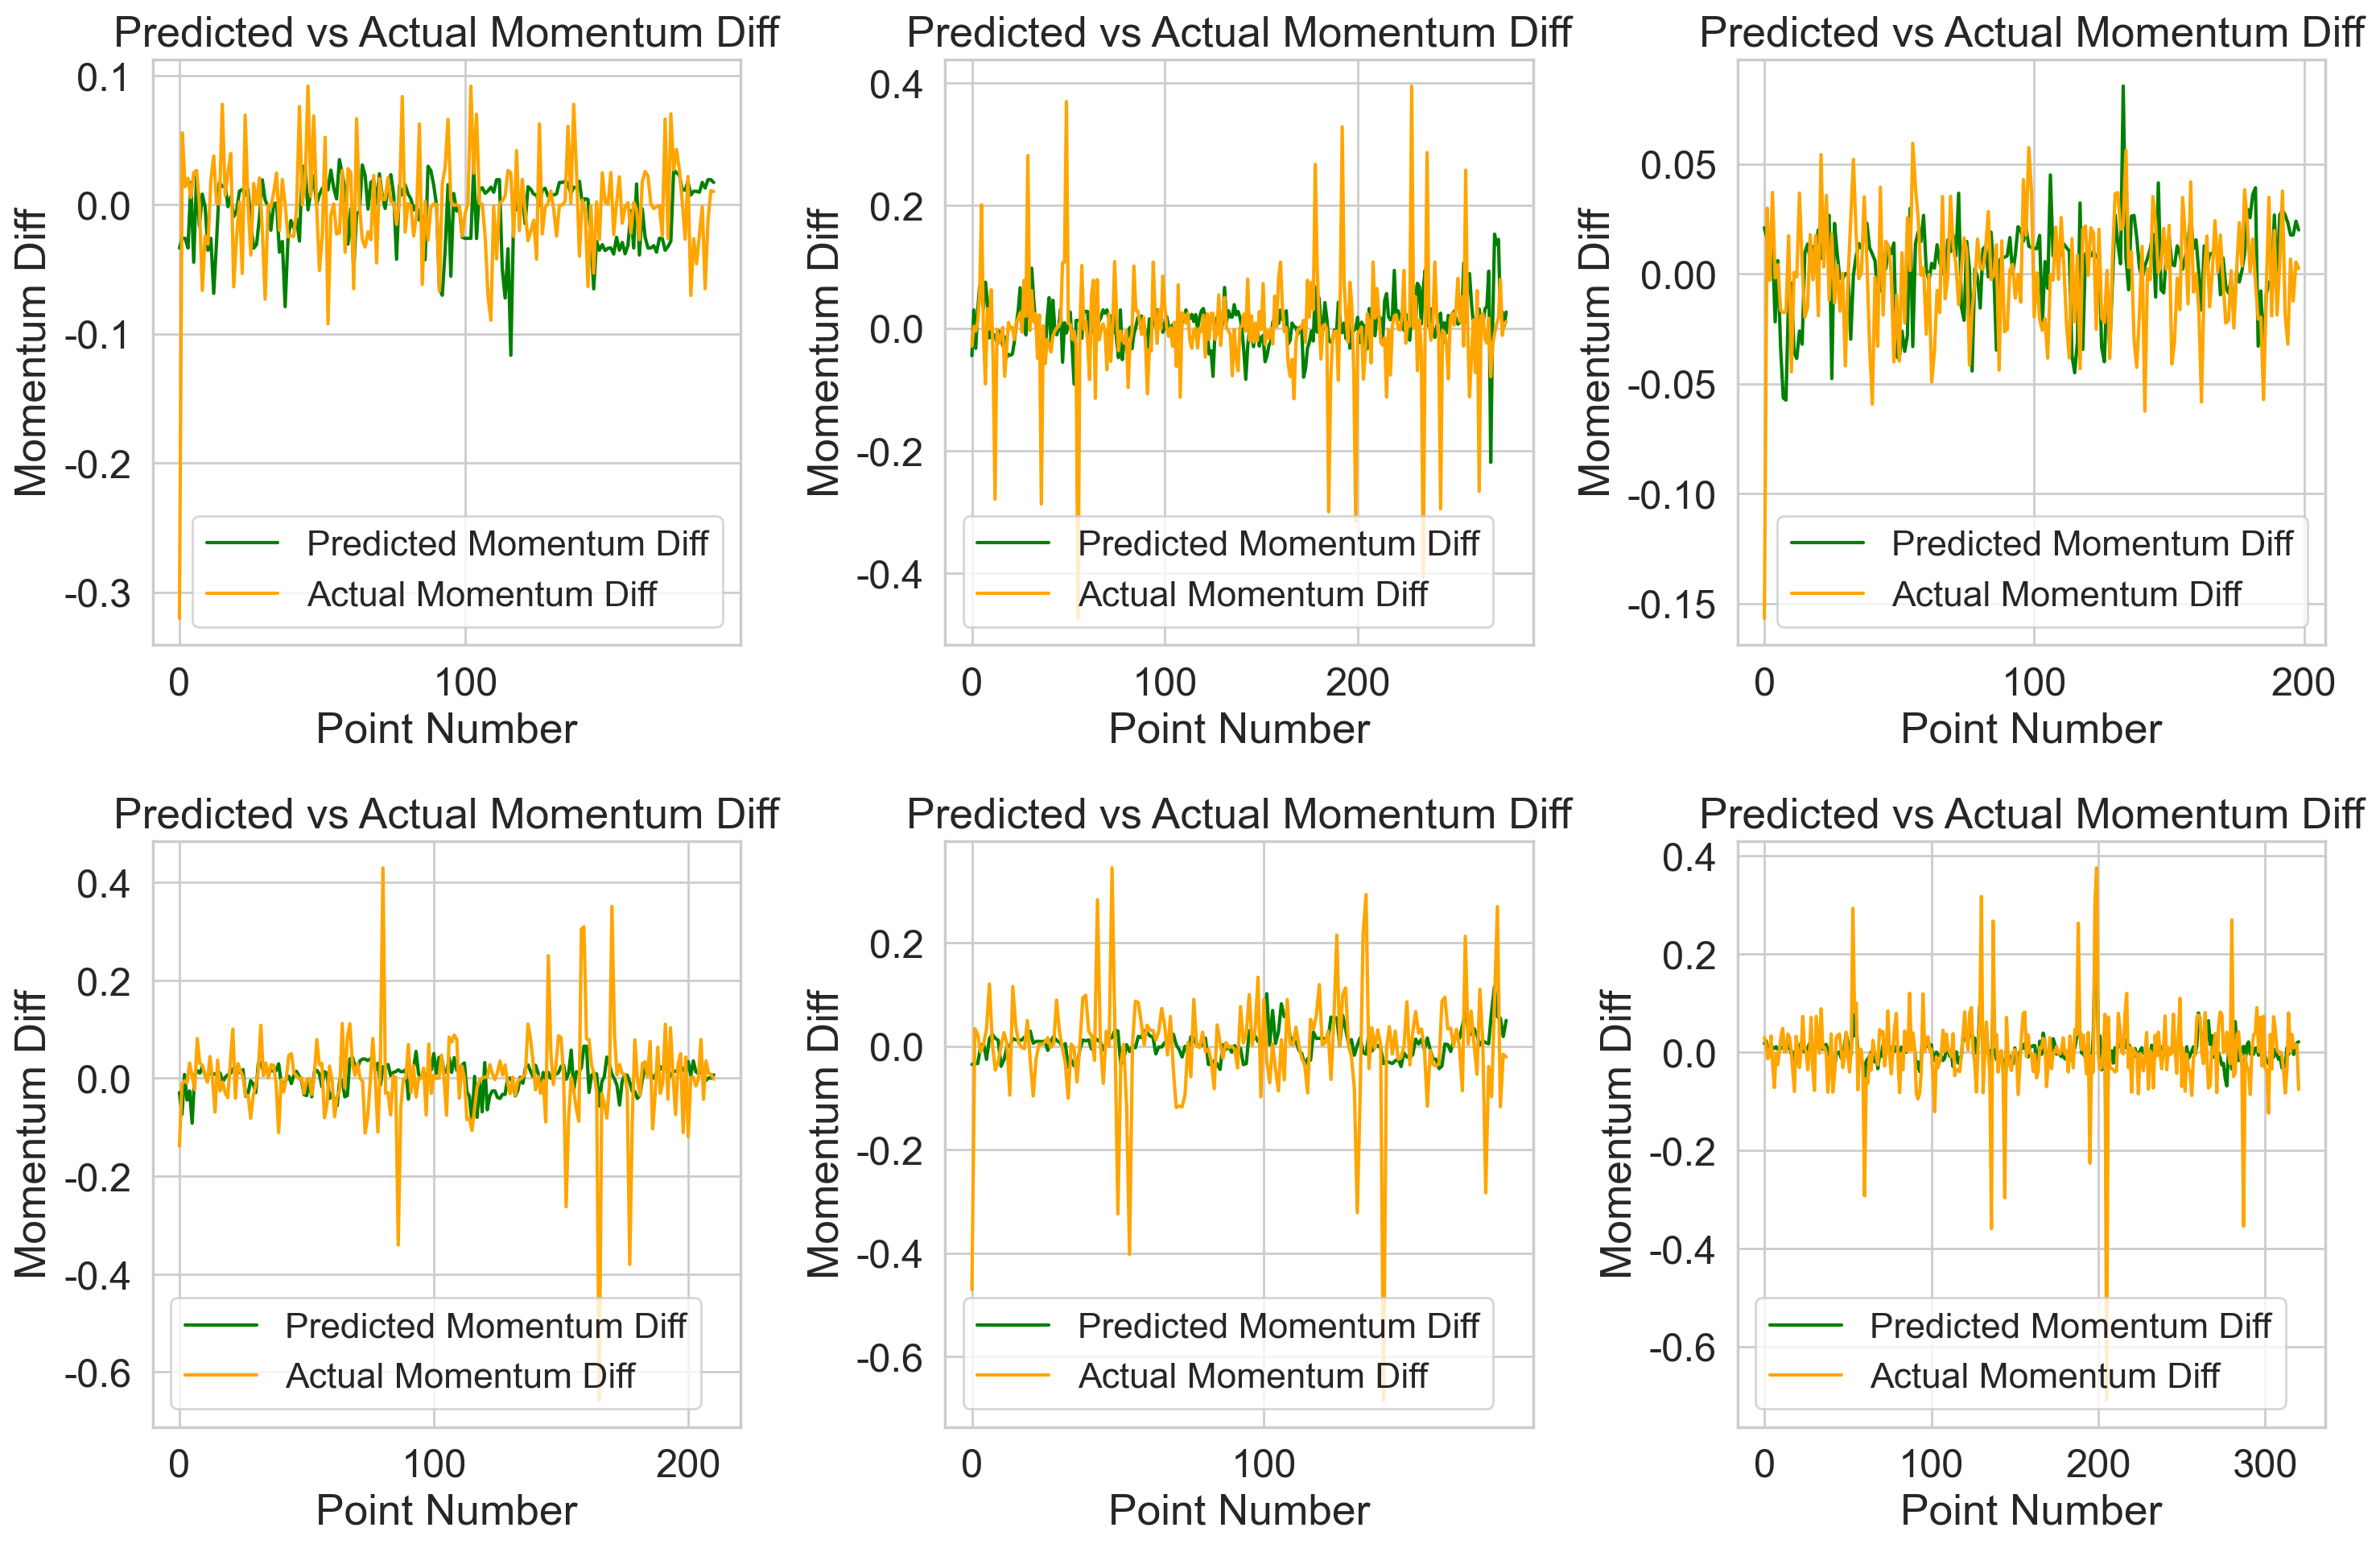
\includegraphics[width=0.75\textwidth, height=0.45\textwidth]{general.png}
    \caption{Prediction of the Difference of the Momentum by XGBoost}
    \label{fig:12}
\end{figure}

\begin{figure}[h!]
    \centering
    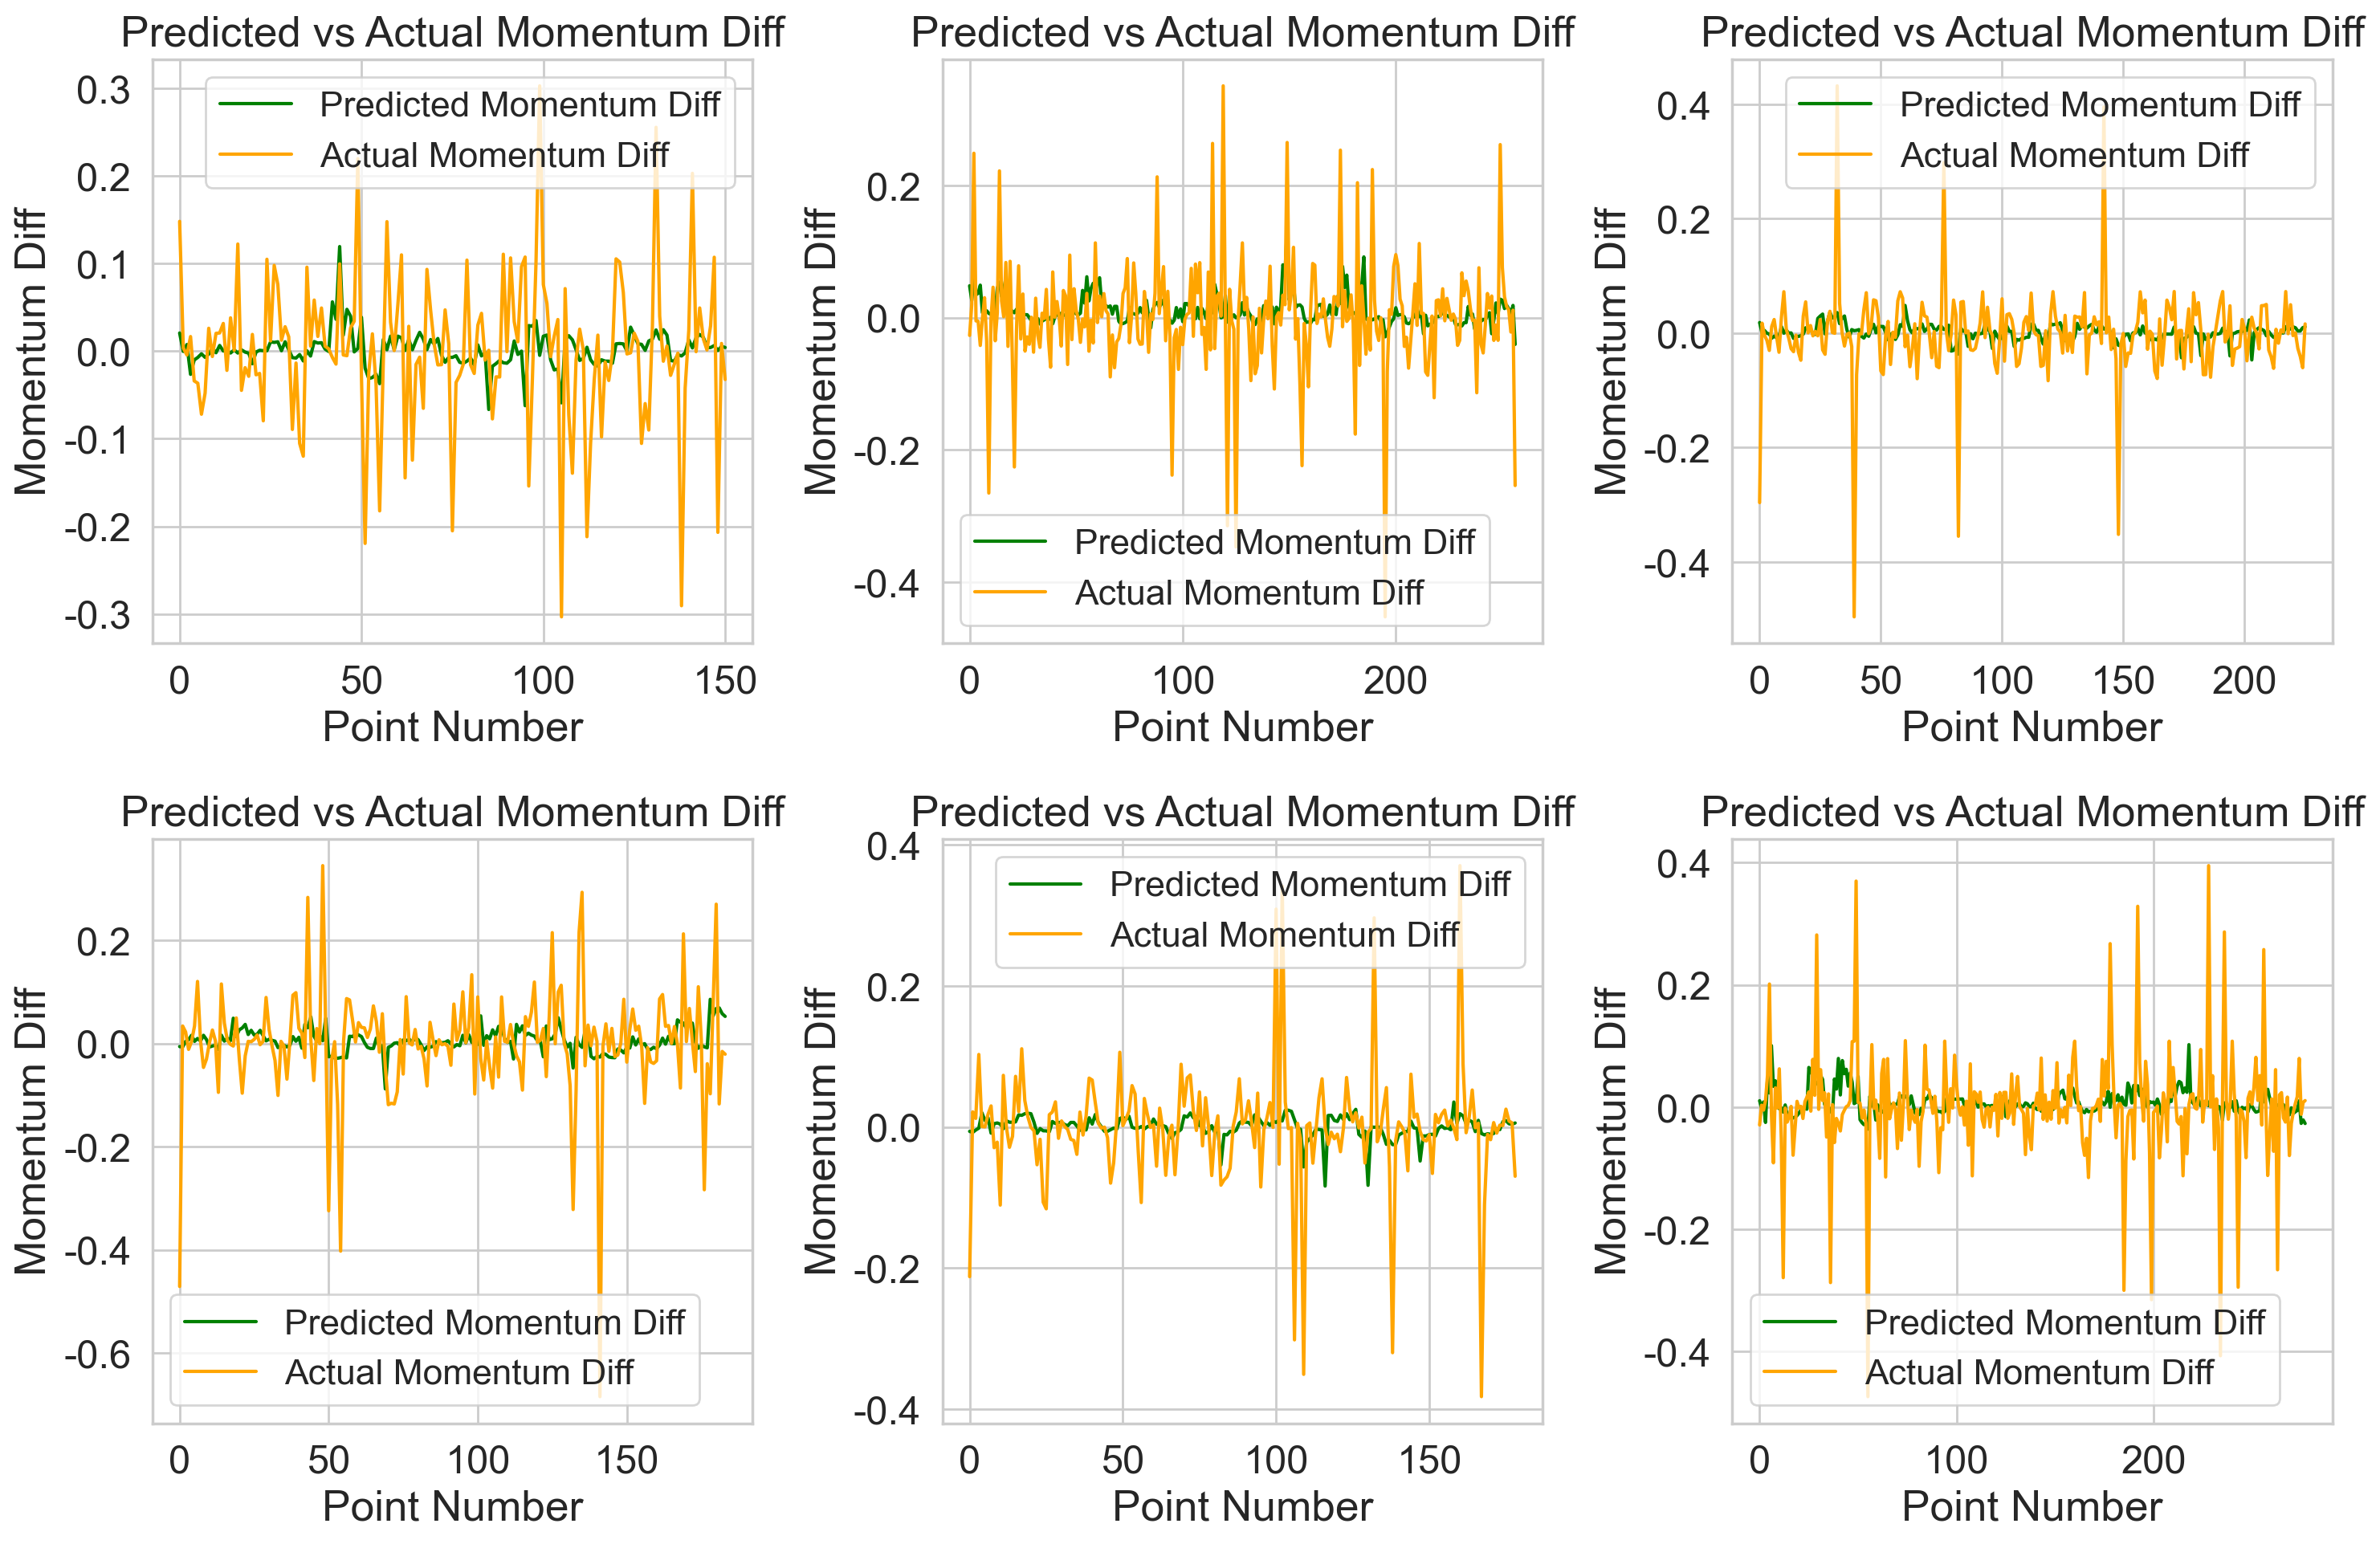
\includegraphics[width=0.75\textwidth, height=0.45\textwidth]{general_lstm.png}
    \caption{Prediction of the Difference of the Momentum by CNN-LSTM}
    \label{fig:13}
\end{figure}

For the XGBoost model, the mean absolute percentage error is about $6.53\%$ and for the CNN-LSTM model, the mean absolute percentage error is $4.41\%$.
It indicates that based on the data of Wimbledon 2023, both models perform a good generality in predicting the difference of the momentum in this tournament.
However, due to the lack of data for the other tournaments or the match of female and mixed doubles, we cannot guarantee our model can still perform well in other tournaments or 
other types of matches. Hence, for predicting other types of matches, we suggest collecting more data on the match and using them to train the model to ensure a better performance since 
during each type of match, the performance of the player might be varied by some different constraints that are not shown in the statistics of the match.

\section{Strength and Weakness}
\subsection{Strength of Our Method}
\quad Through different tests and experiments, we first proved that the outcome of each point can be forecasted by the statistics of the match. Also, our algorithm to quantify the momentum of the player
is proved to be statistically significant. Moreover, we also developed a model to predict the difference of the momentum of the player and the result shows that the model has a good generality and
sensitivity. Because of the advantages of the boosting algorithm model, we can easily interpret which variable has an impact on the momentum of the player.
Therefore, we can conclude that our method can capture the flow of play as points occur and identify which player is performing better at a given time in the match. Also, the feature 
importance of the model is a good reference for the coach to give some insightful advice to the player either to keep a good momentum in the game or prepare for a new game coming up. Moreover, compared to some 
deep learning models that might have better performance in the metric of mean absolute percentage error, the boosting algorithm model is less time-consuming and easier to train with the small dataset. We also 
show in section 5, that even with the limited data of one match, it still can catch the flow of momentum to some extent. As the conditions of players are varied in each match, the statistics of the current match are more 
useful to reflect the performance of the player. Therefore, our method demonstrates a good ability to track the flow of the play in real time.

\subsection{Weakness of Our Method}
\quad As the common criticism of the boosting algorithm model, it's more likely to overfit with the training data. Thus, the generality of the model might be limited and it's hard for it to exactly predict the 
flow of momentum without the finetuning of the model with data of the current match. Moreover, boosting algorithm models like XGBoost and LGBM are not good at capturing the temporal relationship of the input data. 
Although we also tried to use the CNN-LSTM model to capture the temporal relationship and show a relatively low mean absolute percentage error, as the plot shows, the model is not able to capture the trend of the
change of momentum. Also, it is hard to interpret. Therefore, we should be concerned about the trade-off between the performance and interpretability of the model. Finally, we should also keep in mind that  
momentum is more about the psychological state of the player, and the statistics of the match might not be able to fully reflect the psychological state of the player. It's hard for the statistics to capture what a 
player is thinking during the match. Therefore, we can't rely on the prediction of the model to advise the player.

\section{Conclusion}
\quad In this paper, we developed a model to capture the flow of play as points occur and identify which player is performing better at a given time in the match, as well as quantify how much better they are 
performing. We employed the techniques such as cross-validation to make sure the model has good robustness and generality. Also, we applied feature engineering to select the most important variables and used the entropy weight method to
assign weight to each variable to quantify the momentum of the player. By z-score normalization and t-test, we verified the momentum of each player is statistically significant, however, the swing of the play is more likely to be random during
the match. We also developed a model to predict the difference in the momentum of the player and the result supports that the model has an overall good performance and generality. We also extracted the most important features that have a significant 
impact on the momentum of the player and gave some advice to the coach to prepare for the new game. 

However, as we mentioned in the weakness of our model, the model is more likely to overfit with the training data given and it's hard to capture the temporal 
relationship of the input data. Therefore, we suggest collecting more data on the match and using them to train the model to ensure a better performance. Also, we should keep in mind that the momentum is more about the psychological state of the player, 
and in practice some players might give up some points when the opponent's momentum is dominated and save the energy for the next game. Therefore, we can't rely on the prediction of the model to advise the player. As sports are 
more about the people who play them rather than the statistics, it's a bad idea to fully rely on the statistics to predict the outcome of the match. The model we developed is more like a reference instead of a deterministic model to predict the outcome of the match.


\section{Memo Summarizing}

\textbf{To:} Coaches

\noindent\textbf{From:} Team 2426435

\noindent\textbf{Subject:} Advice on momentum and players' response to events that change the flow of play

\vspace{\baselineskip}
\quad The purpose of this memo is to address our team's result of research on momentum in tennis. Our research is based on the data from Wimbledon 2023 men’s matches which shows that the swing of play is not random and we would provide some advice on responding to change in momentum. 

Using some static methodology such as a t-test, we find that the momentum of each player is statistically significant. This result implies that momentum is not random and has an influence on the outcome of the game. 

In our research, we quantify the momentum and use the XGBoost and CNN-LSTM models to perceive the indicators of swing change in the match. As a result, we discover that breakpoint, distance, rally count, and untouchable winning shot have the most influence on momentum. The coach should pay attention to those events and players should respond to them with strategy. 

Here are some advice we have for you based on our research: 
\begin{enumerate}
    \item Breakpoint, based on our analysis, has the most influence on momentum. Thus, we advise player to try their best to earn the best point which would let them gain momentum for the future point. 
    \item If the player loses the breakpoint, most likely the opponent would have a stronger moment than before. Therefore, we recommend players save their energy for the next breakpoint to gain momentum unless they are certain and have the belief they have higher momentum than the opponent. 
    \item Distance and rally count are indicators of the physical exertion of players which also could influence a player's momentum. When the coach and player recognize they are running long distances and have an increase in rally count, they should intentionally control their running distance and rally count to save their momentum.
    \item After a breakpoint or you can recognize the opponent has accumulated their momentum, you could use the tennis technique that increases the opponent's running distance and rally count to reduce the opponent's momentum and gain back or keep the flow of the game in hand. 
    \item Serve also could increase the momentum of the player. Thus, players should use strategy to reduce the momentum of the opponent if they get surve. On the other hand, if the player gets to serve, it is a great opportunity for the player to get the flow of the game back. After the serve, players could use the advice above to maintain the momentum so they could have a high probability of winning. 
    \item Coach should train players' emotional control in day-to-day practice. Momentum is a reflection of human psychology in reality. The player as a human being would be influenced by the momentum. However, if the player has good control of their emotion, they could decrease the negative influence of momentum and increase the positive influence of momentum during the game. 
    \item Coach should actively communicate with the player and recognize the player's momentum changing. Good communication and suggestions of strategy could also increase a player's momentum.
\end{enumerate}

Some factors outside of the court may also affect the performance of the player. For instance, the weather, the condition of the court, the time of the match, or even social media. These factors are 
not included in the dataset and it's hard to quantify the impact of these factors on the performance of each player. Therefore, we suggest coach record the player's statistics in different weather and incorporate them into the dataset for better computational results of the player's momentum. 

All those results and advice are provided based on the Wimbledon 2023 tournament. While our model has a decent generalization, it still has limitations when applied to certain players. Because the 
ability of the player is varied, using more data to train the model may have a good prediction in a general sense but for the specific tournament and player, the model may not perform well. Therefore, we suggest coach  
just use a specific player's data to analyze the indicator of the momentum of that player even if the data is limited. Our experiment shows that limited data will not cause a dramatic decrease in the performance of the model. If you want more accurate momentum changes during the game for a specific player, you could provide your player's statistics data to us. We will be happy to compute the customized result for your player. 

Thank you for taking the time to read our paper. Hope our research can give you some insightful advice to help the player to improve and wish your player could have a good performance in future matches. Feel free to contact us if you have any further questions.

%%%%%%%%%%%%%%%%%%%%%%%%%%%%%%
\printbibliography

%%%%%%%%%%%%%%%%%%%%%%%%%%%%%%
\addcontentsline{toc}{section}{Appendices}
\section*{Appendices}
\addcontentsline{toc}{section}{Appendix A: Selected Feature for Momentum Calculation}
\section*{Appendix A: Selected Feature for Momentum Calculation}
\begin{table}[H]
\centering
\begin{tabular}{|| c ||}
\hline
 \textbf{Variable} \\ [0.5ex] 
    \hline\hline
    Point lead \\
    \hline
    Serve advantage \\
    \hline
    Ace \\
    \hline
    Unforced errors \\
    \hline
    Current leading in sets and games \\
    \hline
    Distance run \\
    \hline
    Break points \\
    \hline
    Untouchable winning shot \\
    \hline
    Rally count \\
    [1ex]
    \hline
\end{tabular}
\caption{Selected Variables}
\label{table:5}
\end{table}

\addcontentsline{toc}{section}{Appendix B: Code For Data Preprocessing}
\section*{Appendix B: Code For Data Preprocessing}
\begin{lstlisting}[style=mystyle, language=Python, caption=, label=]
df = pd.read_csv('Wimbledon_featured_matches.csv')

# data cleaning & preprocessing
df['rally_count'] = df['rally_count'].astype(int)

# convert the elapsed time to seconds
elapsed_seconds = df['elapsed_time'].apply(lambda x: sum(int(a) * 60**index for index, a in enumerate(reversed(x.split(":")))))
df['elapsed_time_sec'] = elapsed_seconds

df.dropna(subset=['speed_mph'],inplace=True)
df.dropna(subset=['serve_width'],inplace=True)
df.dropna(subset=['serve_depth'],inplace=True)

# K-S test for p1_distance_run and p2_distance_run
from scipy.stats import ks_2samp

def ks_test(column_name, list_length = 1000):

    # generate a normal distribution with the same mean and standard deviation of the column we are testing
    mean = df[column_name].mean()
    std = df[column_name].std()
    normal_dist = np.random.normal(mean, std, list_length)

    ks_statistic, p_value = ks_2samp(df[column_name], normal_dist)
    
    return ks_statistic, p_value

# Remove the row with rally_count > 20
df = df[df['rally_count'] <= 20]

# Remove the row with p1_distance_run > 100
df = df[df['p1_distance_run'] <= 100]

# Remove the row with p2_distance_run > 100
df = df[df['p2_distance_run'] <= 100]
\end{lstlisting}

\addcontentsline{toc}{section}{Appendix C: Visualization of Momentum of Players}
\section*{Appendix C: Visualization of Momentum of Players}
\begin{lstlisting}[style=mystyle, language=Python, caption=, label=]
# Plot the monentum of player 1 and player 2 based on points
plt.figure(figsize=(14, 6))

plt.plot(temp['point_no'], temp['p1_momentum'], label=temp['player1'].iloc[0] + " Momentum", color='blue')
plt.plot(temp['point_no'], temp['p2_momentum'], label=temp['player2'].iloc[0] + " Momentum", color='red')

# Horizontal line to show the start of each set
for i in range(1, temp['set_no'].max() + 1):
    plt.axvline(x=temp[temp['set_no'] == i].iloc[0]['point_no'], color='green', linestyle='--')
    plt.text(temp[temp['set_no'] == i].iloc[0]['point_no'], 0, 'Set ' + str(i), verticalalignment='bottom')

plt.legend()
plt.title('Momentum Change Throughout the Match')
plt.xlabel('Point Number')
plt.ylabel('Momentum')

plt.grid(True)
plt.tight_layout()
plt.show()
\end{lstlisting}

\addcontentsline{toc}{section}{Appendix D: Train Test Process in Predicting Point Outcome}
\section*{Appendix D: Train Test Process in Predicting Point Outcome}
\begin{lstlisting}[style=mystyle, language=Python, caption=, label=]
def validation_score(model):
    acc = round(cross_val_score(model,data_point_based[columns].values,data_point_based['point_label'].values, cv=5,scoring='accuracy').mean(),2)
    recall = round(cross_val_score(model,data_point_based[columns].values,data_point_based['point_label'].values, cv=5,scoring='recall').mean(),2)
    precision = round(cross_val_score(model,data_point_based[columns].values,data_point_based['point_label'].values, cv=5,scoring='precision').mean(),2)
    f1 = round(cross_val_score(model,data_point_based[columns].values,data_point_based['point_label'].values, cv=5,scoring='f1').mean(),2)
    auc = round(cross_val_score(model,data_point_based[columns].values,data_point_based['point_label'].values, cv=5,scoring='roc_auc').mean(),2)

    return acc,recall,precision,f1,auc

# Validation score of different models
model_1 = LGBMClassifier(random_state=30,force_col_wise=True)
print(f'LGBMClassifier acc,recall,precision,f1,auc :{validation_score(model_1)}')
model_2 = xgb.XGBClassifier(random_state=50)
print(f'XGBClassifier acc,recall,precision,f1,auc :{validation_score(model_2)}')
model_3 = SVC(random_state=50)
print(f'SVC acc,recall,precision,f1,auc :{validation_score(model_3)}')
model_4 = MLPClassifier(random_state=50)
print(f'MLPClassifier acc,recall,precision,f1,auc :{validation_score(model_4)}')
model_5 = RandomForestClassifier(random_state=50)
print(f'RandomForestClassifier acc,recall,precision,f1,auc :{validation_score(model_5)}')
\end{lstlisting}

\addcontentsline{toc}{section}{Appendix E: Calculate P1's Momentum Criteria and Turning Point}
\section*{Appendix E: Calculate P1's Momentum Criteria and Turning Point}
\begin{lstlisting}[style=mystyle, language=Python, caption=, label=]
def calculate_momentum_improved_P1(df, index, lag=3, serve_advantage_weight = 0.2, ace_weight = 0.2, unforced_error_weight = 0.2):
    start_index = max(index - lag, 0)
    end_index = min(index + lag + 1, len(df))

    df_slice = df.iloc[start_index:end_index]

    # Current leading in sets and games
    p1_sets_won = df_slice['p1_sets'].iloc[-1] - df_slice['p1_sets'].iloc[0]
    p1_games_won = df_slice['p1_games'].iloc[-1] - df_slice['p1_games'].iloc[0]

    # Serve advantage
    p1_serve_advantage = (df_slice[df_slice['server'] == 1]['point_victor'] == 1).sum() * serve_advantage_weight

    # Aces
    p1_aces = df_slice['p1_ace'].sum() * ace_weight

    # Unforced errors
    p1_unforced_errors = -df_slice['p1_unf_err'].sum() * unforced_error_weight

    # Leading points advantage
    p1_points_advantage = df_slice['point_victor'].apply(lambda x: x == 1).sum() - df_slice['point_victor'].apply(lambda x: x == 2).sum()

    # Breaking advantage
    p1_break_points_won = df_slice['p1_break_pt_won'].sum()

    # Untouchable winner
    p1_winners = df_slice['p1_winner'].sum()

    # Distance and rally
    p1_distance = df_slice['p1_distance_run'].sum()
    p1_rally_count = df_slice['rally_count'].sum()

    return p1_sets_won, p1_games_won, p1_serve_advantage, p1_points_advantage, p1_break_points_won, p1_unforced_errors, p1_winners, p1_aces, p1_distance, p1_rally_count

def cumsum_detection(series):

    diff_series = series.diff().fillna(0)
    
    # Calculate the cumulative sum in different series
    cumsum_series = diff_series.cumsum()
    
    # Detect the turning points
    turning_points = []
    for i in range(1, len(cumsum_series)):
        # If the product of the current and previous value is negative, we have a turning point
        if cumsum_series[i] * cumsum_series[i-1] < 0:
            turning_points.append(i)
    
    return turning_points
\end{lstlisting}

\addcontentsline{toc}{section}{Appendix F: Entropy Weight Method}
\section*{Appendix F: Entropy Weight Method}
\begin{lstlisting}[style=mystyle, language=Python, caption=, label=]
def entropy_weight_method(data):
    
    # Standardize the data
    data_normalized = data.apply(lambda x: (x - np.min(x)) / (np.max(x) - np.min(x)))
    
    # Calculate the entropy weight
    epsilon = 1e-12
    p_matrix = data_normalized / data_normalized.sum()
    e_matrix = -np.sum(p_matrix * np.log(p_matrix + epsilon), axis=0) / np.log(len(data))
    
    d_matrix = 1 - e_matrix
    weights = d_matrix / d_matrix.sum()
    
    return weights
\end{lstlisting}

\addcontentsline{toc}{section}{Appendix G: CNN-LSTM Construction}
\section*{Appendix G: CNN-LSTM Construction}
\begin{lstlisting}[style=mystyle, language=Python, caption=, label=]
# Define the model
model = Sequential()
model.add(Conv1D(filters=64, kernel_size=3, activation='relu', input_shape=(X_train.shape[1],1)))
model.add(MaxPooling1D(pool_size=2))
model.add(LSTM(50, activation='sigmoid', return_sequences=True))
model.add(LSTM(50, activation='sigmoid'))
model.add(Dense(1))
model.compile(optimizer='adam', loss='mse')

# Early stopping
es = EarlyStopping(monitor='val_loss', mode='min', verbose=1, patience=5)

# Fit the model
model.fit(X_train, y_train, epochs=100, verbose=1)

# Predict the momentum difference
y_pred = model.predict(X_test)
\end{lstlisting}

\end{document}

